\documentclass[aspectratio=169,11pt]{beamer}
\usepackage{fontspec}
% Aspect ratio:
% 610 => 16:10 
% 169 => 16:9 (Mas común actualmente)
% 149 => 14:9
%  54 => 5:4
%  43 => 4:3 (Default)
%  32 => 3:2

% Tamaño de la fuente
% 8pt, 9pt, 10pt, 11pt (default), 12pt, 14pt, 17pt, 20pt

% Opciones de lenguaje usando polyglossia (defino dos para este documento)
\usepackage{polyglossia}
\setmainlanguage{spanish}
\setotherlanguage[variant=american]{english}

\usepackage{anyfontsize}

% Los símbolos el los conjuntos numéricos
\usepackage{amssymb} 

 % Incluir imágenes
\usepackage{graphicx}
% Poder usar subfiguras
\usepackage{subcaption} 
% Para presentaciones usualmente no necesitamos la primer parte del caption
\captionsetup[figure]{labelformat=empty}
% \captionsetup[table]{labelformat=empty}
\captionsetup[subfigure]{labelformat=empty}
% quitar los simbolos de navegacion
\beamertemplatenavigationsymbolsempty

% Tablas con estilo profesional
\usepackage{booktabs}

% Para usar varias columnas
\usepackage{multicol}

% Para poner algortmos en pseudo código
\usepackage{algpseudocode}
% Ambiente flotante para los algoritmos
\usepackage{algorithm} 
% Hacer los comentarios en el pseudocódigo similares a los de C++
%\algrenewcommand{\algorithmiccomment}[1]{\hskip3em$//$ #1}
% El paquete algorithm, no tiene traducción automática
\floatname{algorithm}{Algoritmo}
\renewcommand{\algorithmicrequire}{\textbf{Entradas:}}
\renewcommand{\algorithmicensure}{\textbf{Salidas:}}
\renewcommand{\listalgorithmname}{Índice de algoritmos}


%Para insertar código fuente en algún lenguaje de programación
\usepackage[newfloat=true]{minted} 
% Requiere que compiles usando:
% $xelatex --shell-escape input.tex

% Configuración del entorno minted para poner código fuente
\DeclareCaptionFormat{mitedFormat}{%
    \textbf{#1#2}#3}
\DeclareCaptionStyle{minetdStyle}{skip=0cm,width=.85\textwidth,justification=centering,
  font=footnotesize,singlelinecheck=off,format=mitedFormat,labelsep=space}
\newenvironment{mintedCode}{\captionsetup{type=listing,style=minetdStyle}}{}
% Cambia el nombre de la etiqueta. Afecta a todos los códigos minted del documento
%\SetupFloatingEnvironment{listing}{name=Código}
\captionsetup[listing]{labelformat=empty}

% Opciones de minted para el lenguaje GLSL
\setminted[glsl]{frame=lines,framesep=0.25cm,baselinestretch=1,fontsize=\scriptsize,breaklines}
% Cuando lo hagas dentro de un párrafo el tamaño de fuente debe ser normal
\setmintedinline[glsl]{fontsize=auto}

% Para usar las comillas en español
\usepackage{dirtytalk}

% Crear un comando con el nombre de la UNAM
\newcommand{\unam}{
  \bfseries
  \normalsize{Universidad Nacional Autónoma de México}
}

% Crear un comando para el email
\newcommand{\email}[1]{
    \texttt{
      \href{https://#1}{#1}
    }
}

% Construyendo la diapositiva de titulo
\title[Shadertoy]{Shaders de Juguete (Shadertoy)}
\subtitle{Usando trucos matemáticos para dibujar en tu navegador web}
\author[Dr. Jorge García]{Dr. Jorge Antonio García Galicia}
\institute[FES Acatlán]{
%     email for contact
    \normalsize{\email{nemediano.github.io}}
%    university name
%    \unam
}
\date[Congreso AI 2025] % (optional)
{Congreso de Inteligencia Artificial, Abril 2025}
\titlegraphic{
\includegraphics[width=1.7cm]{img/escudo-a}}

% Para que el logo parezca en todas las diapositivas
%\logo{
\includegraphics[height=1cm]{img/escudo-a}}

\usetheme{AnnArbor}
\useinnertheme{circles}
\usecolortheme{orchid}
% El tema Annharbor no usa comando de alerta. Los redefinimos
\setbeamercolor{block title alerted}{fg=white,bg=red}
\setbeamercolor{alerted text}{fg=red}

% Definición de colores especiales
\definecolor{azul_unam}{RGB}{0, 43, 122}
\definecolor{dorado_unam}{RGB}{187, 136, 0}
\definecolor{amarillo_quemado}{RGB}{212, 180, 21}

\setbeamercolor{frametitle}{fg=black,bg=amarillo_quemado}
\setbeamercolor{title}{fg=azul_unam,bg=dorado_unam}
\setbeamercolor{title in head/foot}{fg=black,bg=amarillo_quemado}
\setbeamercolor{subsection in head/foot}{fg=azul_unam,bg=dorado_unam}
\setbeamercolor{section in head/foot}{fg=dorado_unam}
\setbeamercolor{author in head/foot}{fg=dorado_unam}
\setbeamercolor{institute in head/foot}{fg=dorado_unam}
\setbeamercolor{page number in head/foot}{fg=azul_unam,bg=dorado_unam}
\setbeamercolor{date in head/foot}{fg=azul_unam,bg=dorado_unam}

% Pongo linkcolor vacío para que los links internos no tengan color
% Solo los links externos tienen color
\hypersetup{colorlinks,linkcolor=,urlcolor=azul_unam}

\setbeamertemplate{caption}{\insertcaption}

\begin{document}
% Primer slide contiene el título
\begin{frame}{}
    \maketitle
\end{frame}
% El contenido de la presentación esta en estos documentos
\section{Introducción}
\begin{frame}{¿Qué esperar del taller?}
\begin{columns}
\column[t]{0.5\textwidth}
    \begin{itemize}
         \item Aprender el paradigma de \href{https://iquilezles.org/articles/nvscene2008/rwwtt.pdf}{Rendering Worlds With Two Triangles}.
         \item Parte del \href{https://www.smu.edu/meadows/newsandevents/news/2023/what-is-creative-coding}{creative codding}: intersección entre el arte y la ciencia.
         \item Un poco de \href{https://www.khronos.org/opengl/wiki/OpenGL_Shading_Language}{GLSL}, y las matemáticas básicas para hacer un \href{https://www.khronos.org/opengl/wiki/Portal:OpenGL_Shading_Language/Fragment_Shader}{fragment shader} en el paradigma.
     \end{itemize}
\column[t]{0.5\textwidth}
\begin{figure}[htp]
 \centering
 \begin{subfigure}[b]{0.42\textwidth}
   
\includegraphics[width=\textwidth]{img/Demo/SwirlyWhirly}
   \caption{\href{https://www.shadertoy.com/view/X3dBRr}{Swirly Whirly}}
 \end{subfigure}
~
 \begin{subfigure}[b]{0.42\textwidth}
   \includegraphics[width=\textwidth]{img/Demo/SelfieGirl}
   \caption{\href{https://www.shadertoy.com/view/WsSBzh}{Selfie Girl}}
 \end{subfigure}
\\
 \begin{subfigure}[b]{0.42\textwidth}
   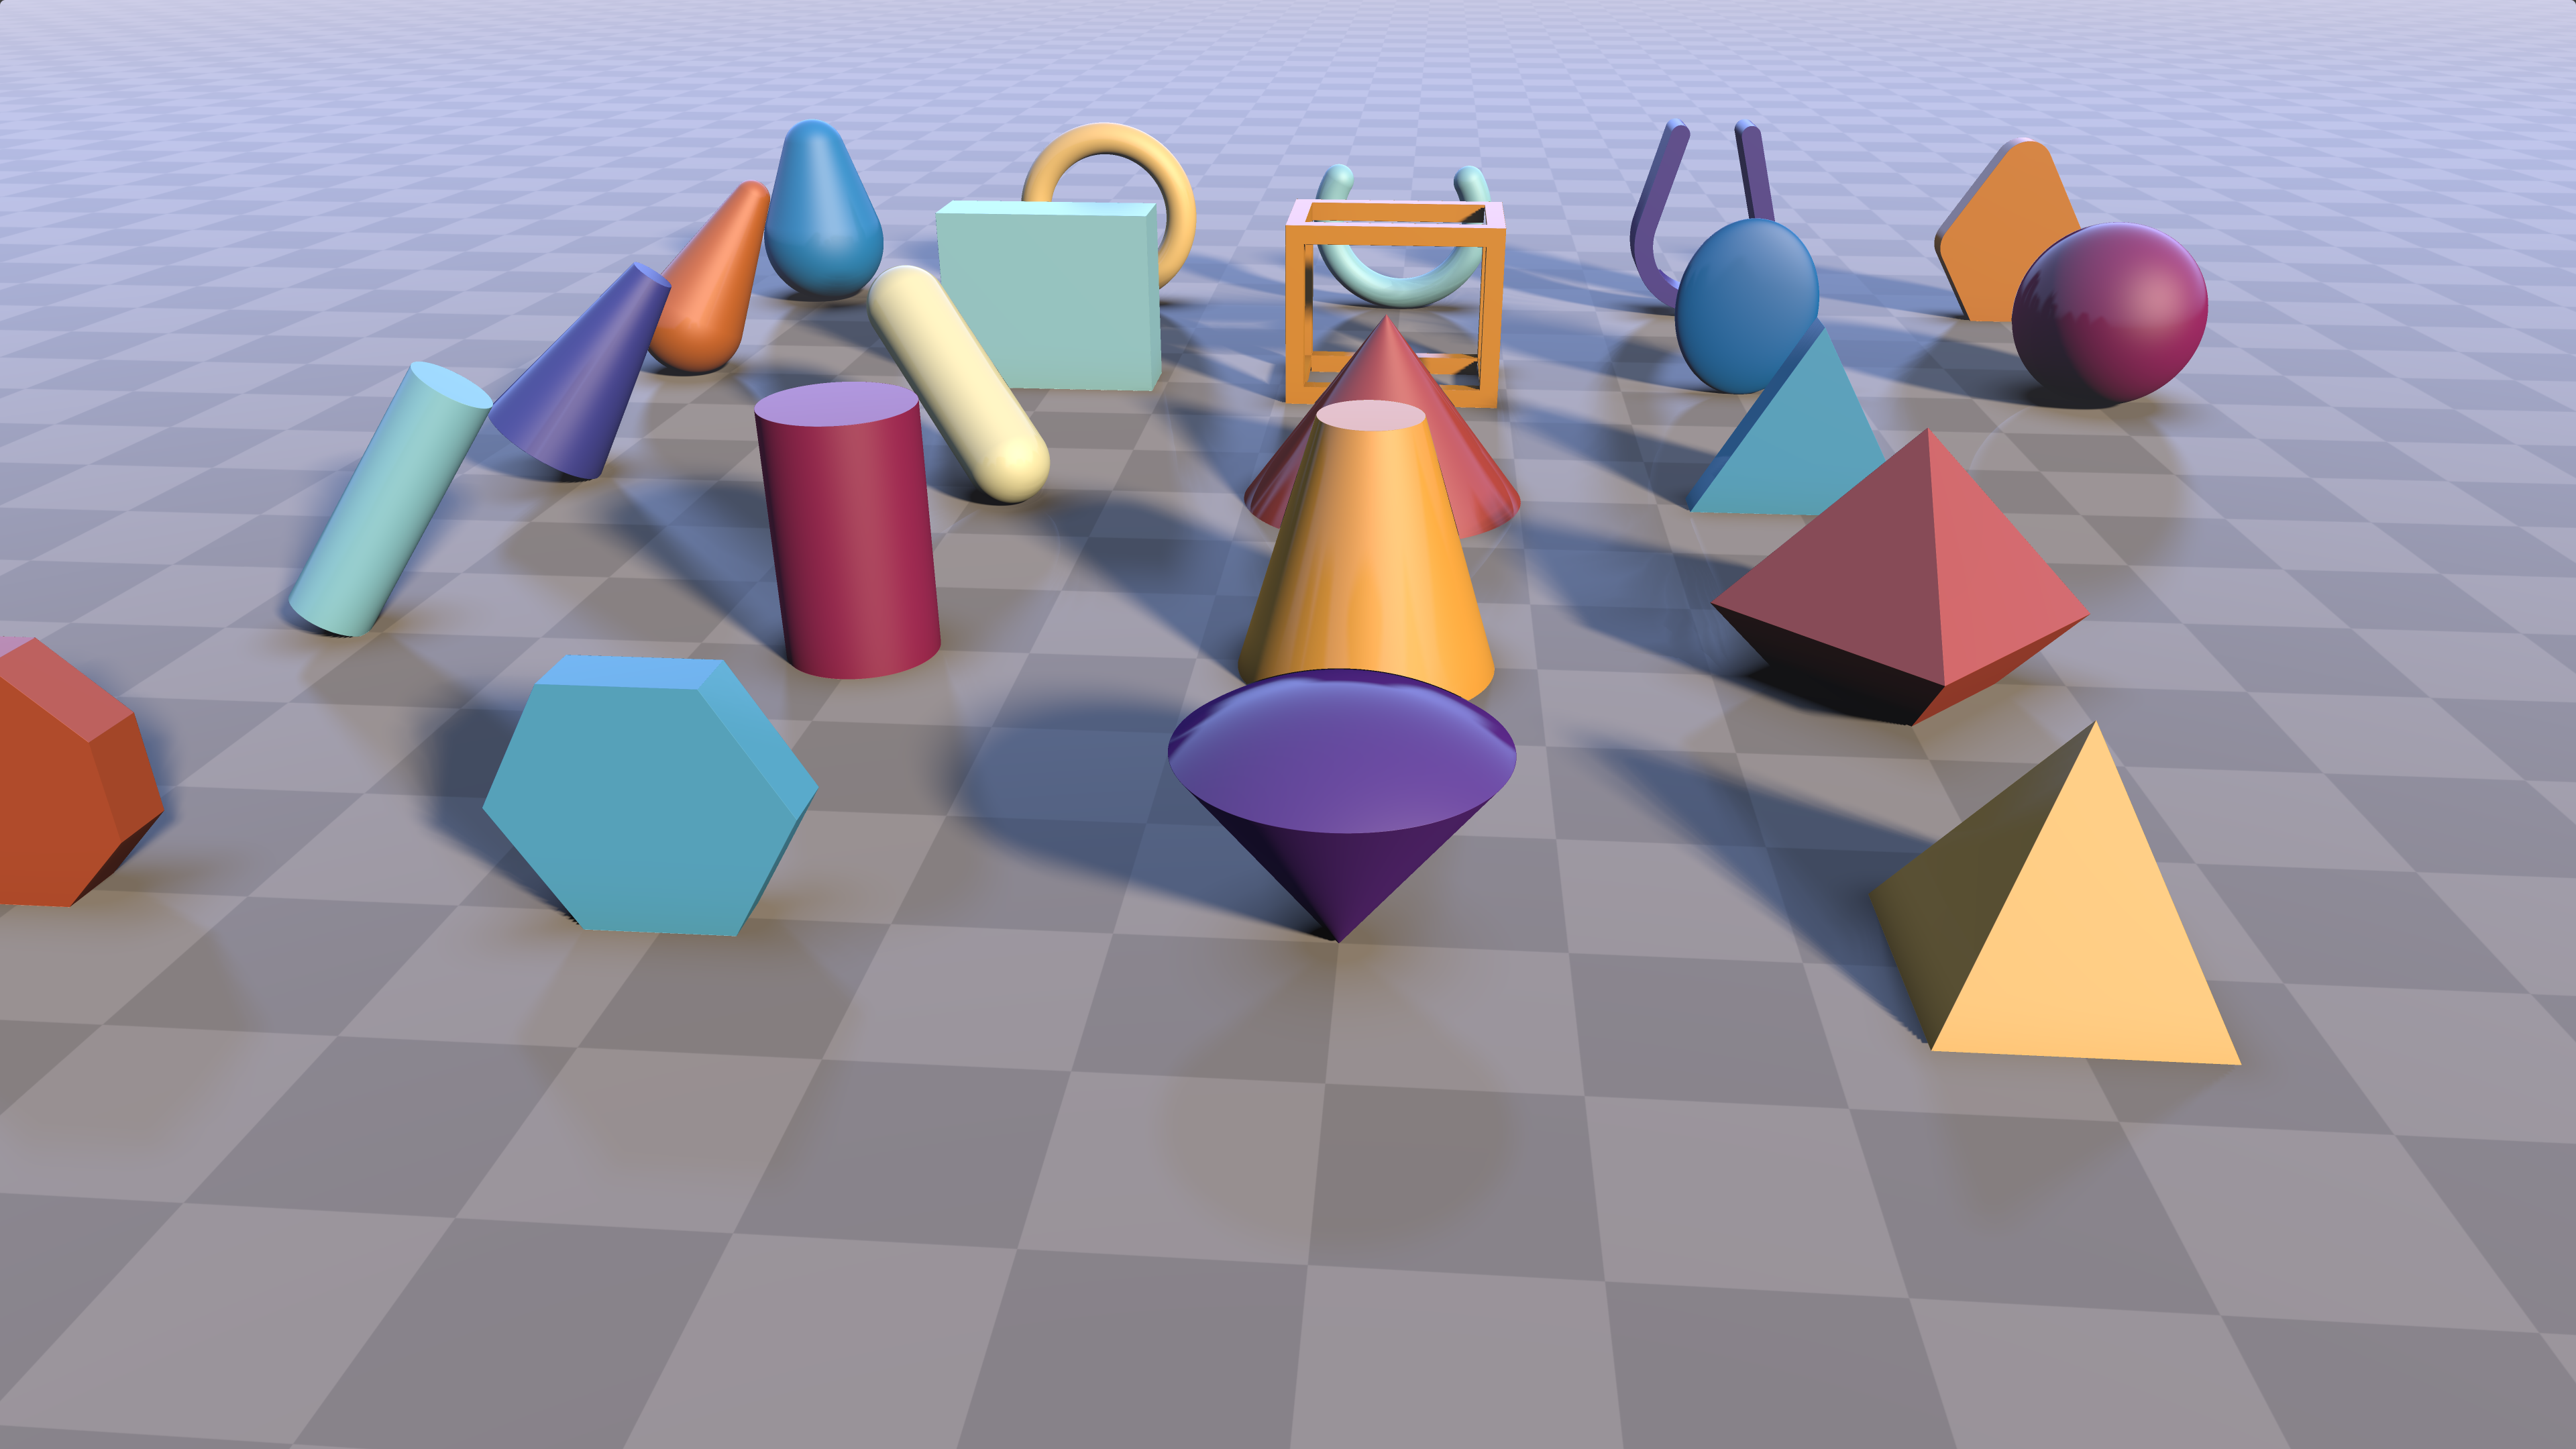
\includegraphics[width=\textwidth]{img/Demo/Raymarching-Primitives}
   \caption{\href{https://www.shadertoy.com/view/Xds3zN}{Raymarch Primitives}}
 \end{subfigure}
~
 \begin{subfigure}[b]{0.42\textwidth}
   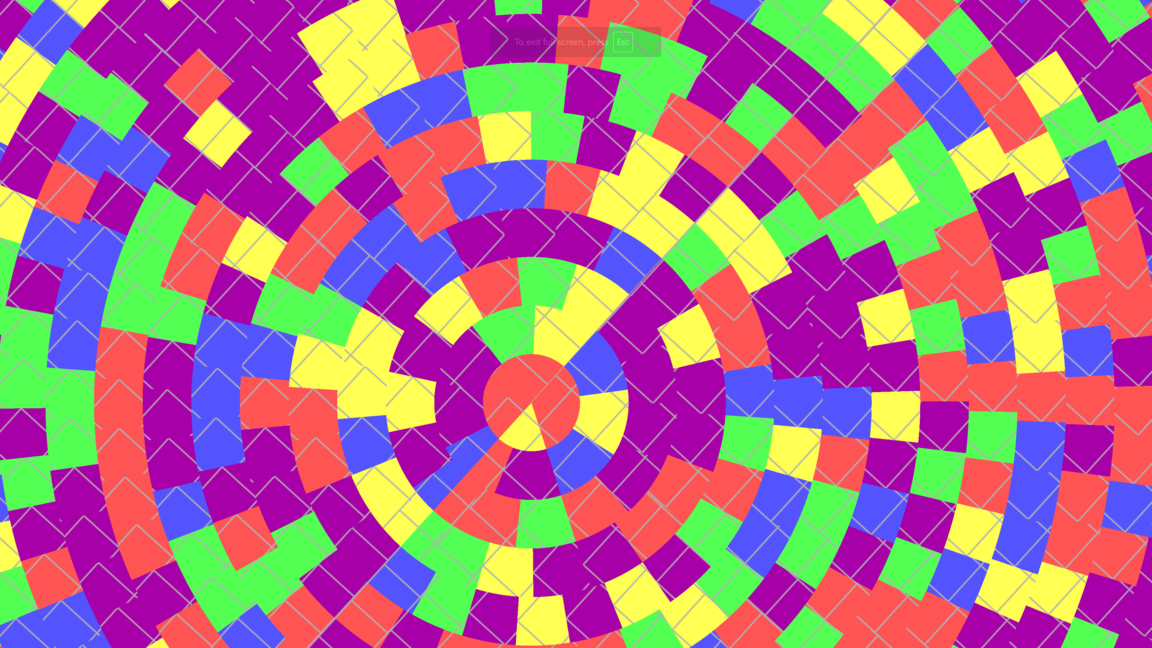
\includegraphics[width=\textwidth]{img/Demo/AnimatedCentricMosaicTiles}
   \caption{\href{https://www.shadertoy.com/view/43tfRr}{Centric Mosaic Tiles}}
 \end{subfigure}
 \caption{Propiedad de los respectivos autores.}
\end{figure}
\end{columns}
\end{frame}

\begin{frame}{¿Qué \emph{no es} éste taller?}
    No es un curso \emph{completo} de \say{Graficación por Computadora}.
    Mas aun, no vamos a enseñar a hacer gráficas por computadora de manera correcta.
    \begin{itemize}
         \item Usar este paradigma \alert{es un juego}. No se usa en producción.
         \item Los shaders que vamos a escribir son ineficientes.
         \item El código puede ser ofuscado.
     \end{itemize}
     Por razones de tiempo, tampoco enseñaremos todo lo que hay en el truco.
     \begin{block}{}
         \begin{itemize}
            \item Este es un taller \alert{básico} de shaders de juguete (Shadertoy).
            \item Revisaremos un conjunto de técnicas simples.
            \item Recuerda: hacer shaders complejos, requiere de experiencia, creatividad y tiempo.
        \end{itemize}  
    \end{block}
\end{frame}

\begin{frame}{¿Qué puedo aprovechar de éste taller?}
    \begin{itemize}
         \item Aprender una manera de expresión artística usando programación.
         \item Un excelente ejercicio para fomentar la creatividad.
         \item Una forma de practicar, aplicar y mejorar tus conocimientos de matemáticas y de computación.
         \item Un medio de compartir con una comunidad (Shadertoy tiene elementos de red social).
         \item Se convierte en un hobby productivo.
     \end{itemize}
     
     \begin{block}{Graficación por Computadora}
         \begin{itemize}
            \item Una probadita para saber si estas interesado en tomar un curso formal después.
            \item Si ya tomaste el curso, es un \emph{hack} muy elegante que seguramente no se te había ocurrido.
            \item Muchos profesionales del área lo practican como hobby.
        \end{itemize}  
    \end{block}
\end{frame}

\begin{frame}{Acerca de mí}
    \begin{columns}
\column[t]{0.5\textwidth}
        \begin{figure}[htb]
            \centering
            
\includegraphics[width=0.6\textwidth]{img/Avatar12}
            \caption{Dr. Jorge Antonio García Galicia.}
        \end{figure}
\column[t]{0.5\textwidth}
     \begin{itemize}
         \item \href{https://mac.acatlan.unam.mx/}{Licenciatura} y \href{https://www.pcic.unam.mx/}{maestría} en la \href{https://www.unam.mx/}{UNAM}.
         \item \href{https://polytechnic.purdue.edu/degrees/phd-technology}{Doctorado} en \href{https://www.purdue.edu/}{Purdue University}.
         \item Hice una pasantía en \href{https://research.adobe.com/}{Adobe} y trabajé en \href{https://www.nvidia.com/}{Nvidia}.
         \item He dado clases en \href{https://www.acatlan.unam.mx/}{Acatlán} y fui ayudante en \href{https://www.fciencias.unam.mx/directorio/63922}{Ciencias} y en \href{https://polytechnic.purdue.edu/}{Purdue}.
         \item Actualmente soy SWE en \href{https://about.google/}{Google}.
         \item Tengo mas de 15 años de experiencia en Tecnología.
     \end{itemize}
\end{columns}
\end{frame}

\begin{frame}{Mi experiencia con gráficos}
\begin{columns}
\column[t]{0.5\textwidth}
    \begin{itemize}
         \item Tres tesis que tienen que ver con \href{https://en.wikipedia.org/wiki/Computer_graphics}{Graficación por Computadora}.
         \item Publicado en \href{https://direct.mit.edu/leon}{Leonardo}, \href{https://www.siggraph.org/}{SIGGRAPH} y en \href{https://www.eg.org/wp/eurographics-publications/}{Eurographics}.
         \item Trabajé en el driver de \href{https://www.opengl.org/}{OpenGL} y en \href{https://stadia.google.com/gg/}{Stadia}.
         \item Actualmente trabajo en \href{https://www.android.com/xr/}{AndroidXR}.
         \item Provengo de una familia de artistas.
     \end{itemize}
\column[t]{0.5\textwidth}
\begin{figure}[htp]
 \centering
 \begin{subfigure}[b]{0.4\textwidth}
   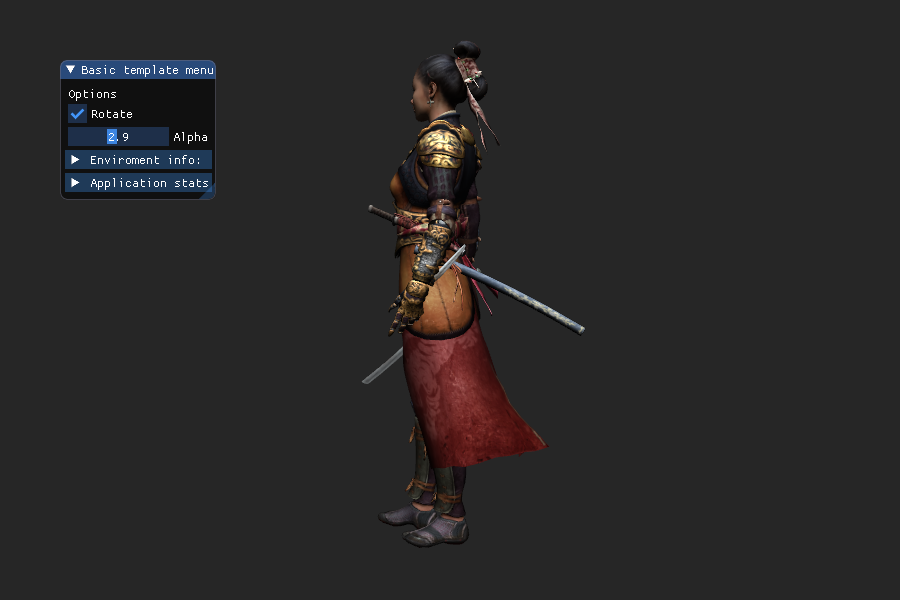
\includegraphics[width=\textwidth]{img/menuTemplate}
 \end{subfigure}
~
 \begin{subfigure}[b]{0.4\textwidth}
   
\includegraphics[width=\textwidth]{img/completo}
 \end{subfigure}
\\
 \begin{subfigure}[b]{0.4\textwidth}
   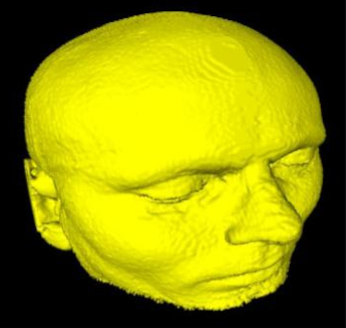
\includegraphics[width=\textwidth]{img/master}
 \end{subfigure}
~
\begin{subfigure}[b]{0.4\textwidth}
   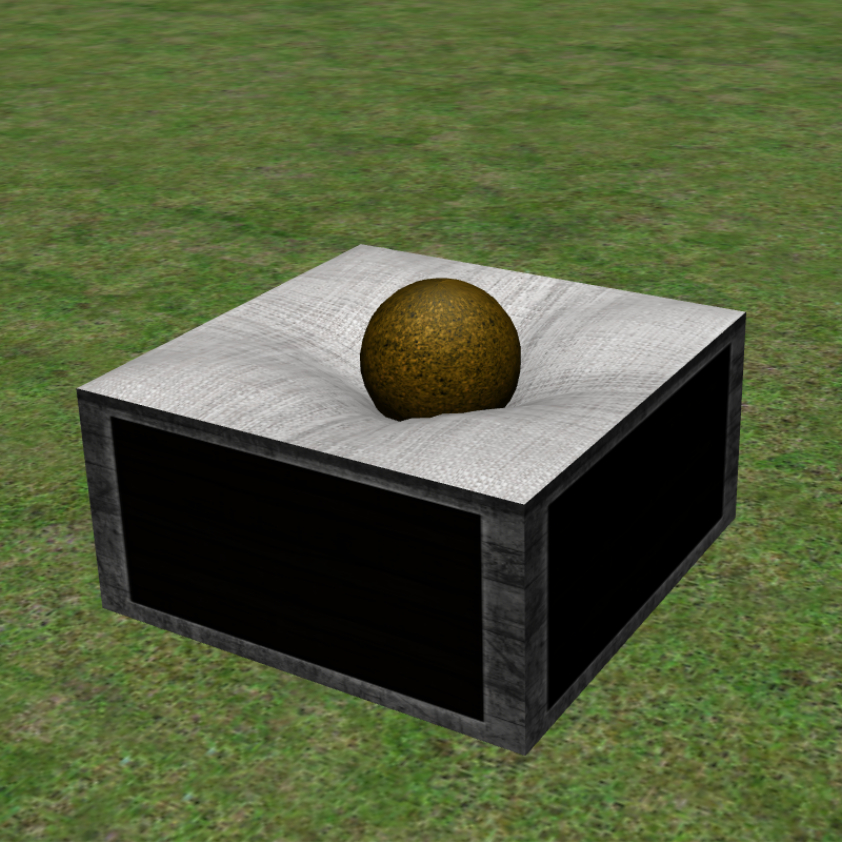
\includegraphics[width=\textwidth]{img/bachelor_thesis}
 \end{subfigure}
 
\end{figure}
\end{columns}
\end{frame}

\section{Gráficas por computadora actualmente}

\begin{frame}{El GPU}
\begin{block}{Graphics processing unit (GPU)}
    Un procesador programable con alta capacidad de computo en paralelo, que generalmente opera con imágenes digitales.
\end{block}
    \begin{itemize}
        \item Originalmente estaba dedicado a hacer gráficos.
        \item Actualmente, hace computo general, de hecho es el \href{https://en.wikipedia.org/wiki/AI_accelerator}{AI acelerator} mas usado.
        \item No confundir con una tarjeta de video: Todas la tarjetas de video (actuales) tiene un GPU. Pero no todos los GPU están en tarjetas de video.
        \item Cuando un GPU esta físicamente separado del chip que tiene el CPU se le llama un GPU discreto.
     \end{itemize}
\end{frame}

\begin{frame}{¿Qué es un shader?}
\begin{block}{Shader}
    Un programa que es ejecutado de manera paralela en el GPU como parte de un pipeline.
\end{block}
Acerca del nombre:
    \begin{itemize}
        \item El termino fue acuñado por Pixar en 1988 para Renderman.
        \item Originalmente (2001), los shaders solo hacían cálculos de iluminación: intensidad de la luz, color, sombras y brillos.
        \item De ahí su nombre, que significa \emph{sombreado}.
     \end{itemize}

\end{frame}

\begin{frame}{La pieza básica}
\begin{block}{Pipeline gráfico.}
    Es una abstracción de SW, que describe el proceso que debe seguir un programa para trasformar una escena tridimensional en una imagen.
\end{block}
\begin{figure}[htb]
  \centering
  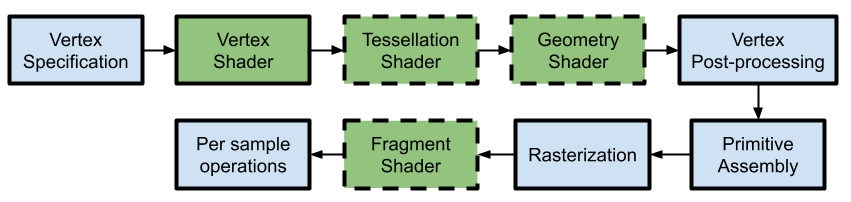
\includegraphics[width=0.7\textwidth]{img/RenderPipeline}
\end{figure} 
\end{frame}

\begin{frame}{Simplificando\ldots}
\begin{itemize}
    \item El la práctica, los tesselation shaders y los geometry shaders solo se usan para cosas muy especificas.
    \item Mas aún, casi nunca se configuran los estados entre el vertex shader y la rasterización.
    \item Para propósitos de esta explicación, podemos pensarlo de manera mas simple:    
\end{itemize}
\begin{figure}[htb]
  \centering
  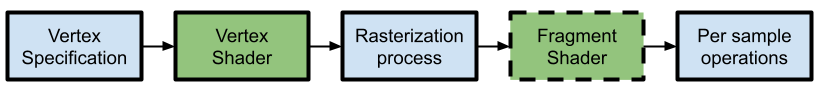
\includegraphics[width=0.7\textwidth]{img/SimplifiedPipeline}
\end{figure}
\end{frame}

\begin{frame}[allowframebreaks]{¿Cómo se programa una aplicación gráfica?}
\begin{itemize}
    \item En general tienes que usar al menos tres cosas:
    \begin{enumerate}
        \item Un lenguaje de programación en el CPU para crear una aplicación.
        \item Un API gráfico, para construir, configurar y conectar el pipeline.
        \item Un lenguaje para escribir shaders.
    \end{enumerate}
    \item En este taller solo escribiremos código de shaders usando \href{https://www.khronos.org/opengl/wiki/OpenGL_Shading_Language}{GLSL}.
    \item Pero sin darnos cuenta el navegador de hecho usa: \href{https://en.wikipedia.org/wiki/JavaScript}{javascript} y \href{https://www.khronos.org/webgl/}{WebGL}, que es un \href{https://www.khronos.org/opengles/}{subconjunto de OpenGL}.
\end{itemize}
\begin{figure}[htb]
  \centering
  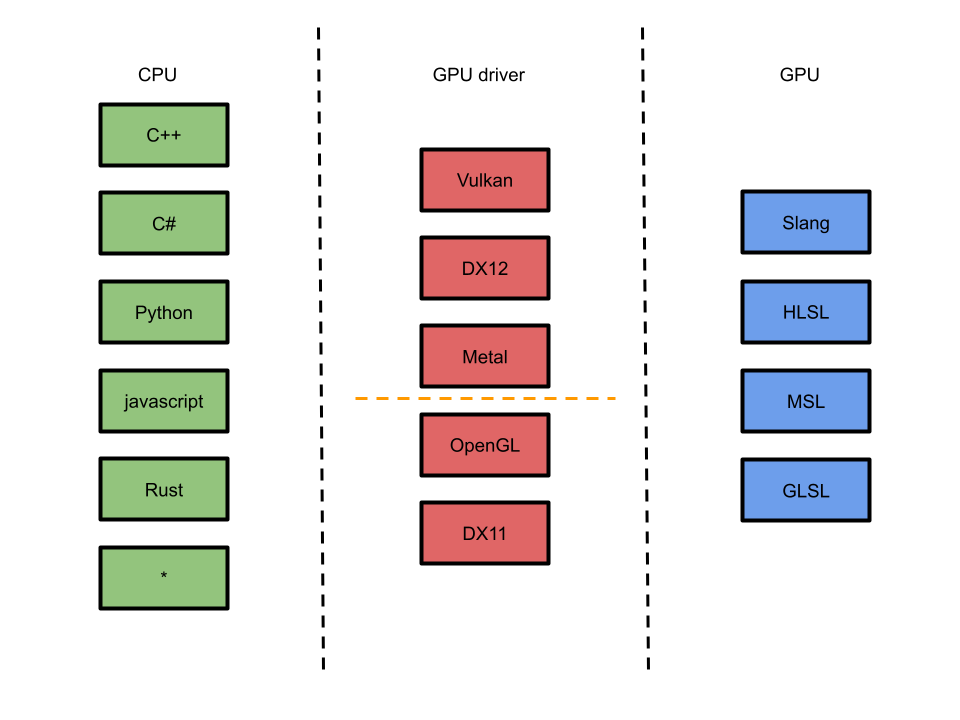
\includegraphics[width=0.6\textwidth]{img/APIs}
  %\caption{Hay varias opciones para cada caso}
\end{figure}
\end{frame}

\begin{frame}[allowframebreaks]{Anatomía de una aplicación}
Actualmente, una aplicación típica:
    \begin{itemize}
        \item Esta escrita en un engine gráfico (Como \href{https://unity.com/}{Unity} o \href{https://www.unrealengine.com/}{Unreal}).
        \item Para producir un frame, se usan cientos de pipelines.
        \begin{itemize}
            \item Varios pipelines, producen resultados en texturas que luego otros pipelines consumen.
            \item Cada material de los objetos de la escena tiene su propio pipeline.
            \item Hay pipelines especializados en ciertas tareas (Sombras, reflexiones, iluminación, etc.).
            \item Algunos son directos, otros diferidos, otros por mosaicos.
            \item Sin contar que muchos efectos se llevan a cabo en compute shaders.
        \end{itemize}
    \end{itemize}
    \begin{figure}[htb]
        \centering
        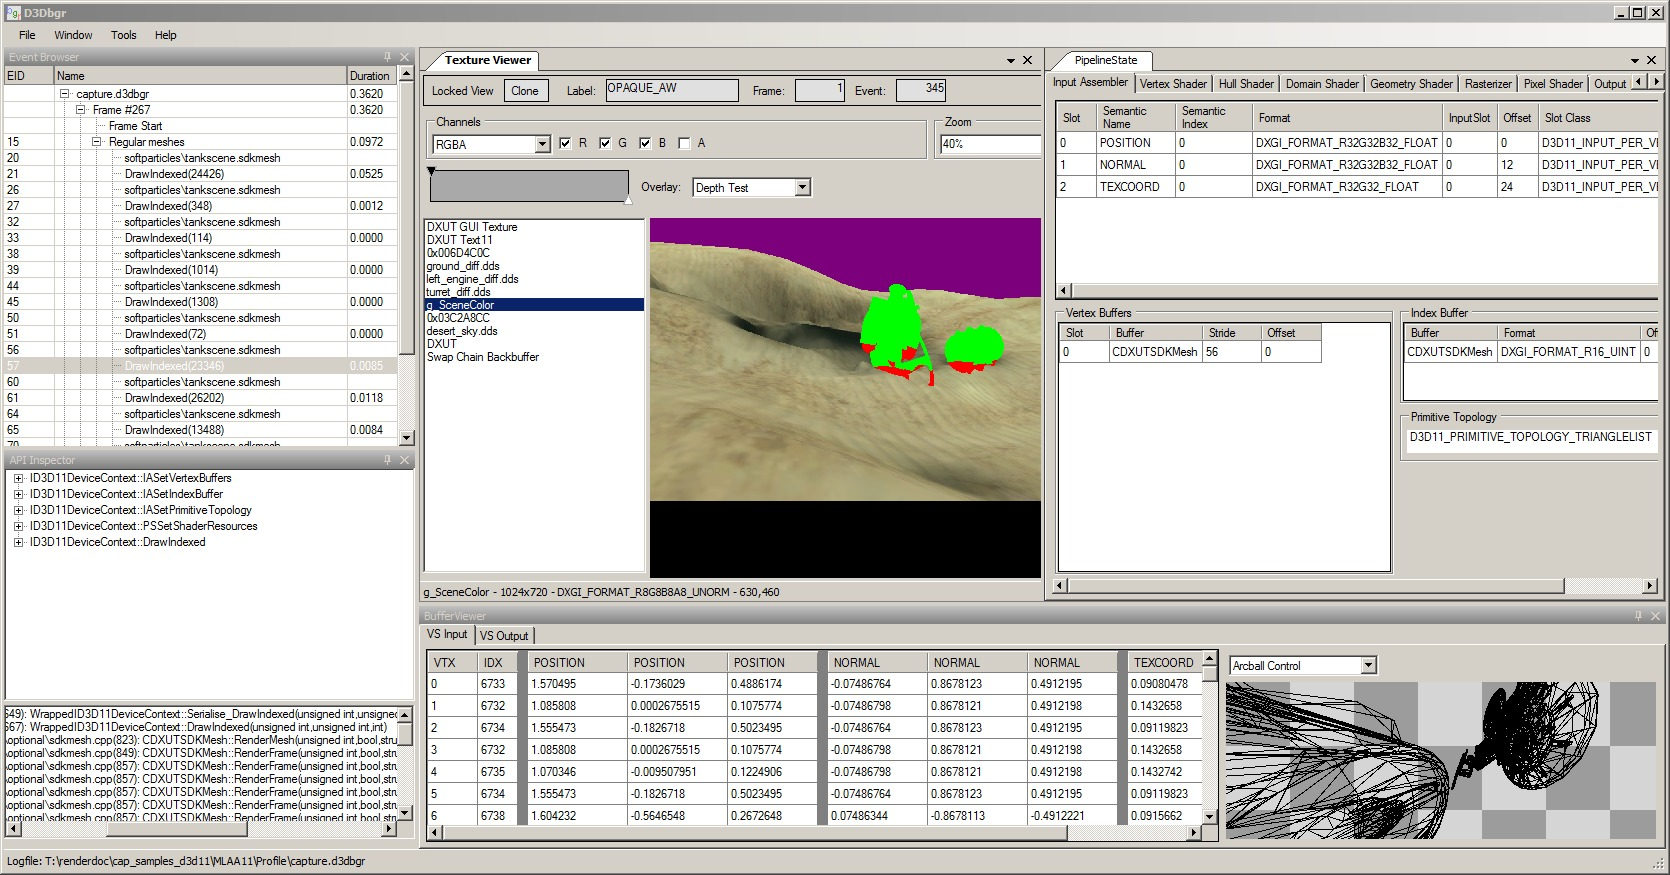
\includegraphics[width=0.8\textwidth]{img/functionality}
    \end{figure}
\end{frame}

\begin{frame}{¿Qué nos depara el futuro?}
\begin{columns}
\column[t]{0.5\textwidth}
    Hay una tendencia importante hacia:
    \begin{itemize}
        \item Unificar en el modelo de \href{https://en.wikipedia.org/wiki/Physically_based_rendering}{iluminación PBR}.
        \item Las técnicas basadas en rayos: \href{https://en.wikipedia.org/wiki/Path_tracing}{Pathtracers}.
        \begin{itemize}
            \item Generar parte de los fragments de un frame (o incluso frames completos), \href{https://www.youtube.com/watch?v=5PHBXY0FI5o&t=2s}{usando técnicas de AI} en vez de calcularlos.
        \end{itemize}
        \item Definir un nuevo pipeline: Task (Amplification) shaders, \href{https://www.khronos.org/blog/mesh-shading-for-vulkan}{Mesh shaders}.
        \item Descargar la mayor parte de las tareas en el \href{https://en.wikipedia.org/wiki/Compute_kernel}{Compute shader}.
    \end{itemize}
\column[t]{0.5\textwidth}
\begin{figure}[htp]
  \centering
  \includegraphics[width=0.6\textwidth]{img/pathtracer}
\end{figure}
\end{columns}
\end{frame}


\section{Shadertoy}

\begin{frame}{Una idea ingeniosa}
Todo empezó con una \href{https://iquilezles.org/articles/nvscene2008/rwwtt.pdf}{plática}: \say{Rendering Worlds With Two Triangles} presentada en la \href{https://www.youtube.com/watch?v=A1iW6Z_Jc4k}{conferencia NVScene} el 22 Aug 2008 por \href{https://iquilezles.org/}{Iñigo Quilez}
\begin{exampleblock}{}
\begin{enumerate}
    \item Si dibujamos un cuadrado (formado por 2 triángulos), que cubre toda la ventana. Esto provocará la ejecución del fragment (pixel) shader en todos los píxeles de la pantalla. 
    \item Luego, usamos el fragment shader en donde cada fragment (pixel) sabe su respectiva posición en el render target, unas constantes (uniforms) y un montón de matemáticas, para dibujar la escena.
\end{enumerate}
\end{exampleblock}
\begin{figure}[htp]
  \centering
  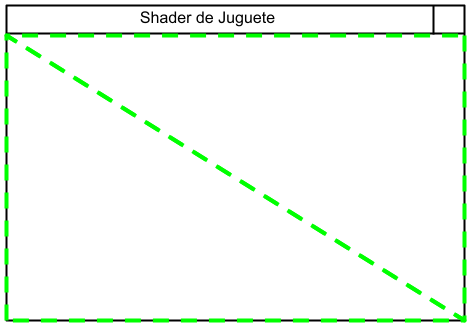
\includegraphics[width=0.2\textwidth]{img/TwoTriangles}
\end{figure}
\end{frame}

\begin{frame}{Regresar al principio}
\begin{figure}[htp]
  \centering
  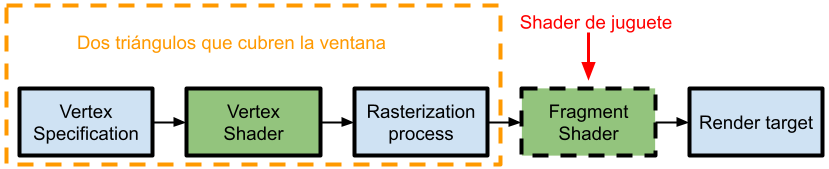
\includegraphics[width=0.7\textwidth]{img/Truco}
\end{figure}
\begin{itemize}
    \item Es similar a como se hacían los gráficos antes de que tuviéramos tarjetas de video.
    \item Solo que ahora aprovechamos el \alert{inmenso poder paralelo} del GPU
    \item Y usamos GLSL
\end{itemize}
\end{frame}

\begin{frame}{Nota curiosa}
\begin{figure}[htp]
  \centering
  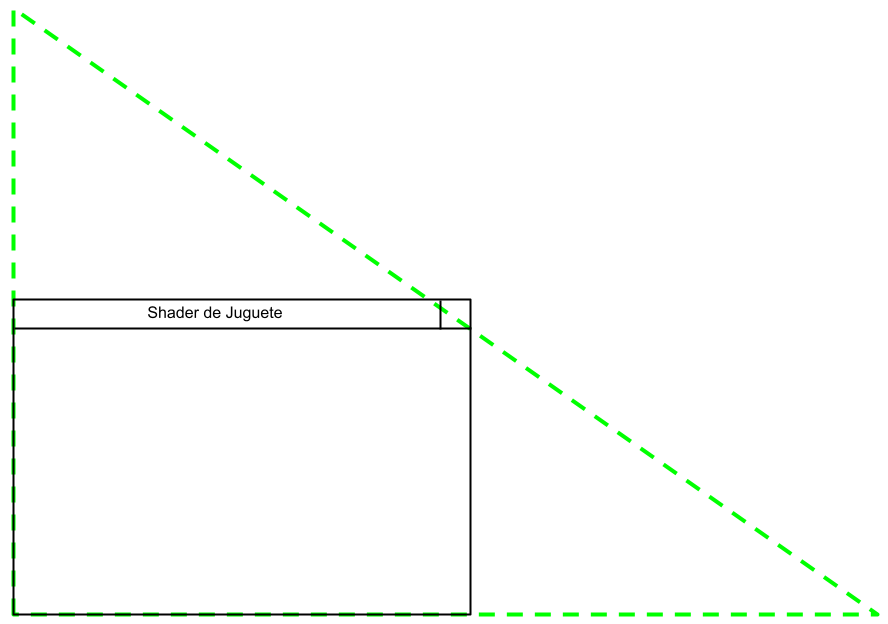
\includegraphics[width=0.4\textwidth]{img/onetriangle}
\end{figure}
De hecho podemos hacerlo con un solo triángulo y luego hacemos clipping.
\end{frame}

\begin{frame}{Actualmente, es mejor hacer:}
\begin{figure}[htp]
  \centering
  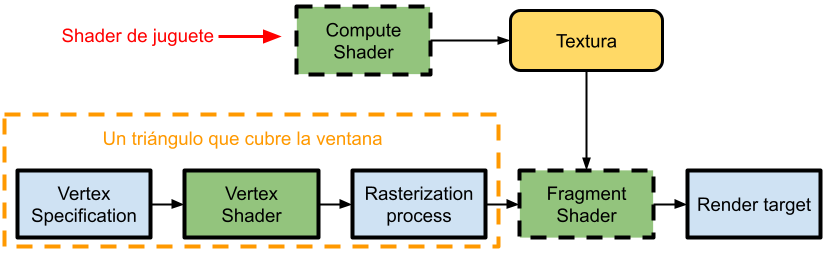
\includegraphics[width=0.65\textwidth]{img/TrucoModerno}
\end{figure}
\end{frame}

\begin{frame}{Shadertoy}
\begin{itemize}
    \item Shadertoy es un sitio web: \url{https://www.shadertoy.com/} que nos da la infraestructura para usar el truco
    \item Y ciertas herramientas sociales
    \item Fue creado por \href{https://iquilezles.org/}{Iñigo Quilez} y \href{https://www.poljeremias.com/}{Pol Jeremias} en el 2013
\end{itemize}
\begin{figure}[htp]
  \centering
  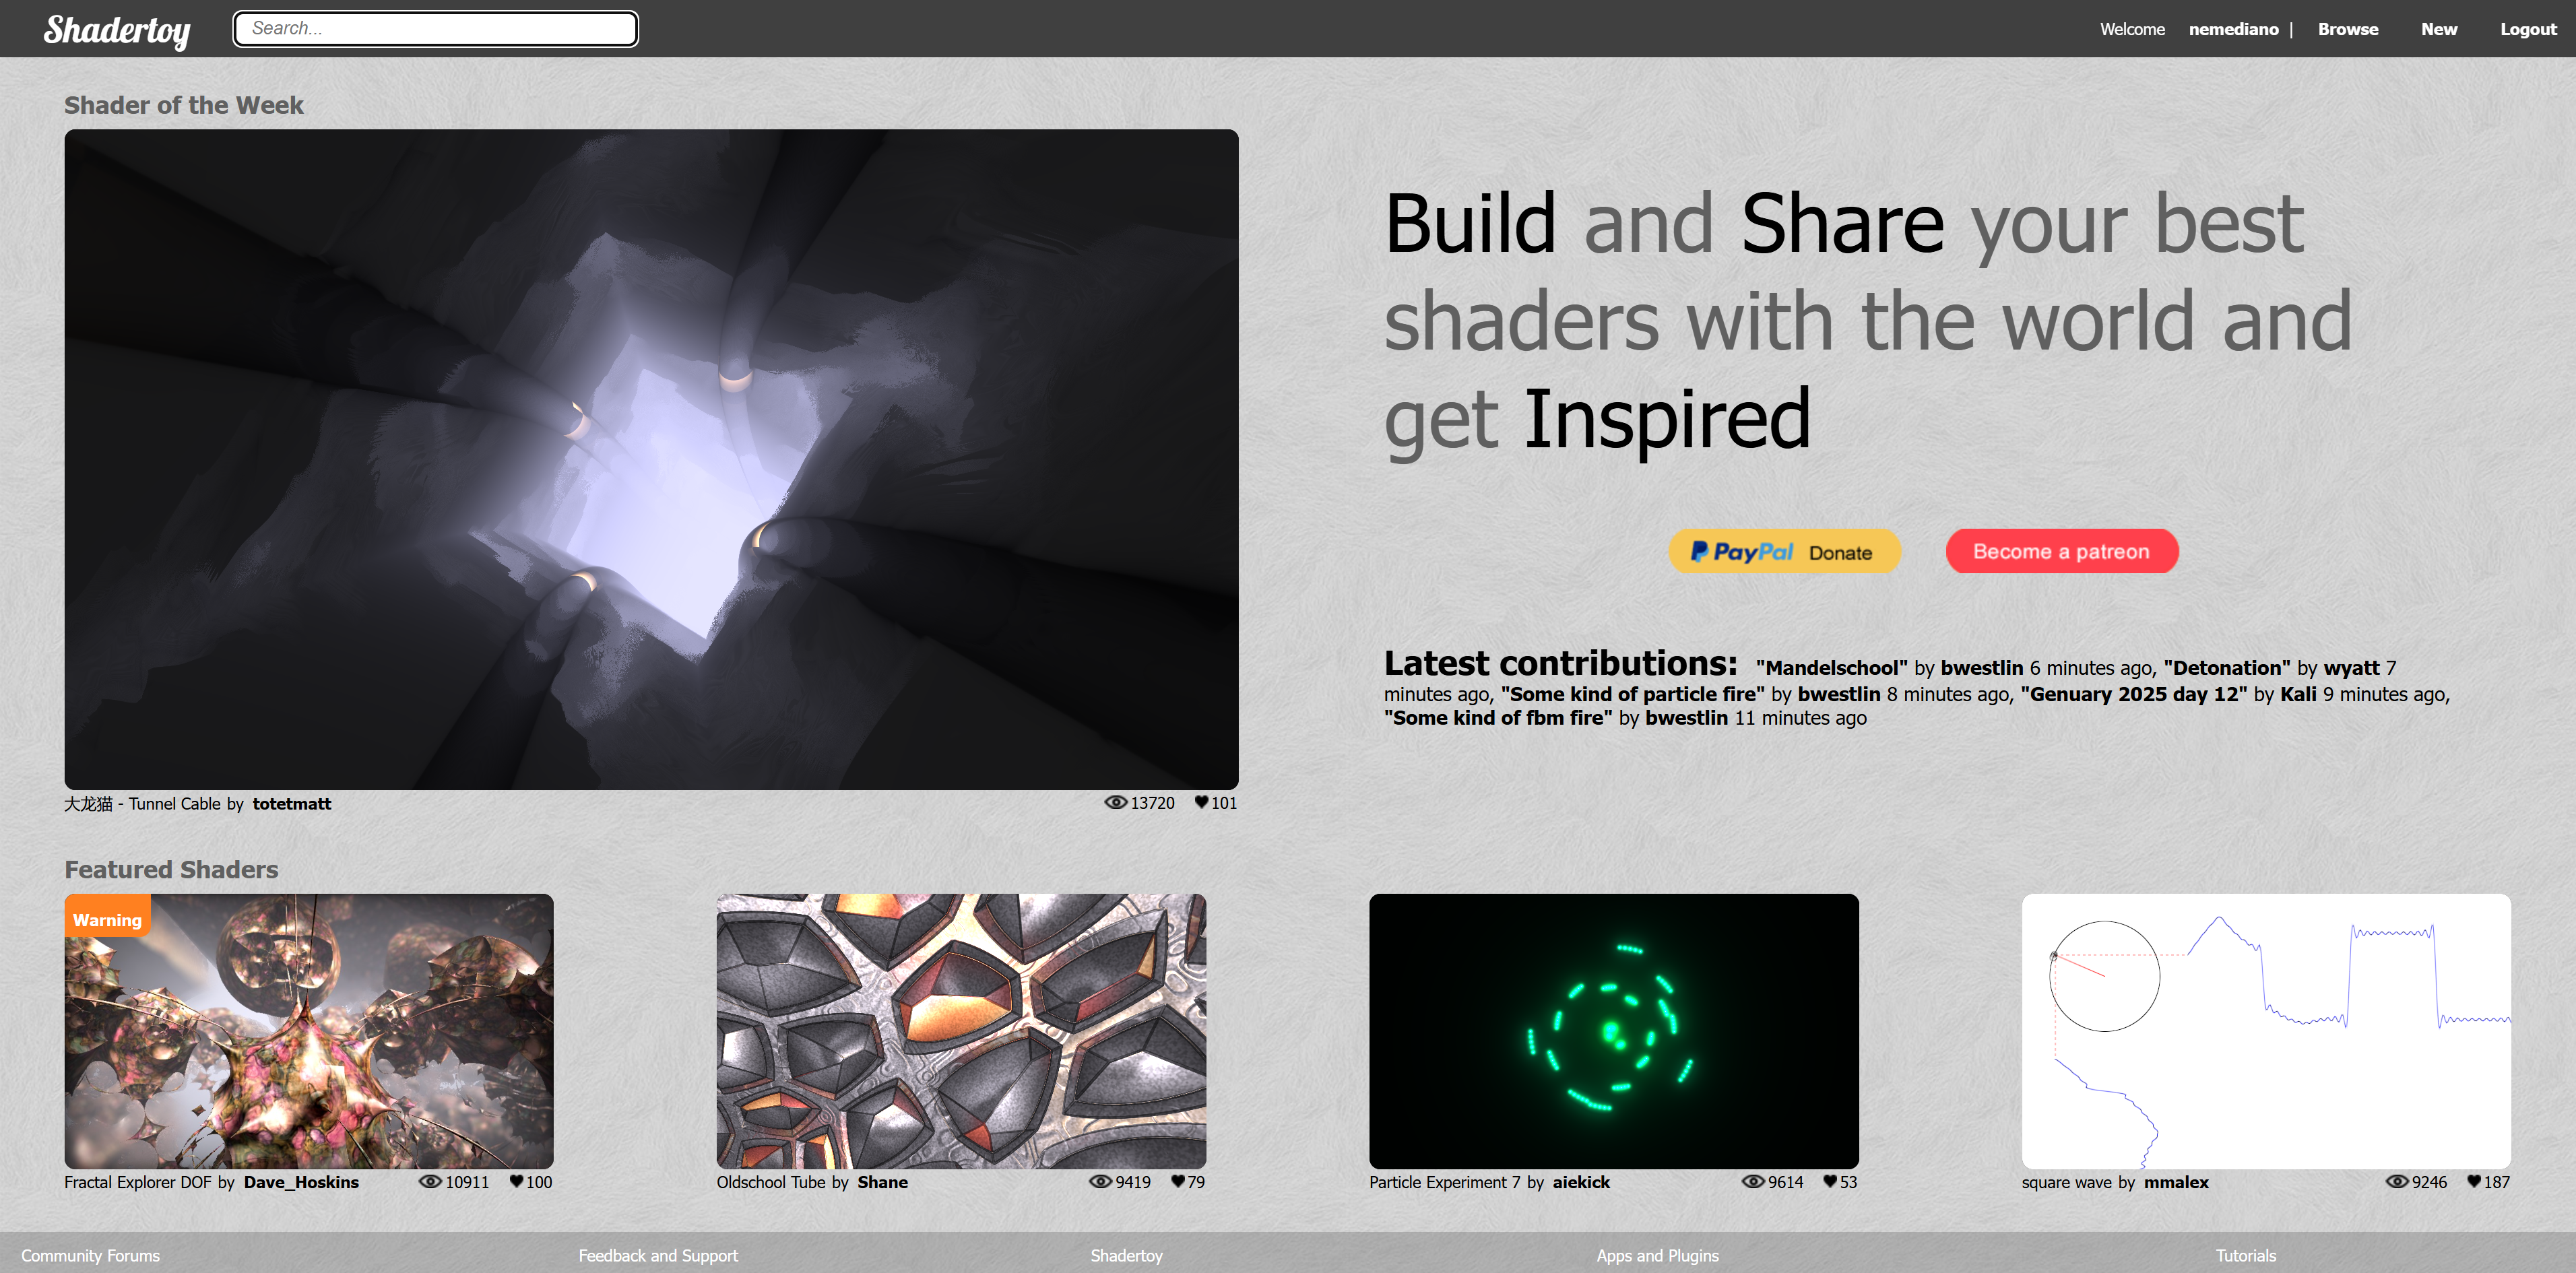
\includegraphics[width=0.4\textwidth]{img/ShaderToySite}
\end{figure}
\end{frame}

\begin{frame}{¿Cómo se usa?}
Escribir un programa en \href{https://www.khronos.org/opengl/wiki/Core_Language_(GLSL)}{GLSL} que se ejecuta en paralelo por cada pixel de la salida.
\begin{itemize}
    \item \textbf{Entradas:} recibes la coordenada del pixel
    \item \textbf{Salida:} debes regresar el color del pixel
    \item Recibe algunas constantes extra: el tiempo, el tamaño total del render target, etc.
\end{itemize}
\begin{figure}[htp]
  \centering
  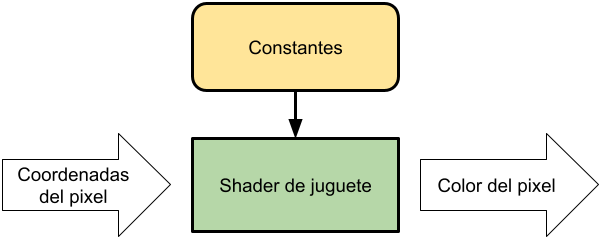
\includegraphics[width=0.4\textwidth]{img/SimpleShaderToy}
\end{figure}
\end{frame}

\begin{frame}{Así se ve}
\begin{figure}[htp]
  \centering
  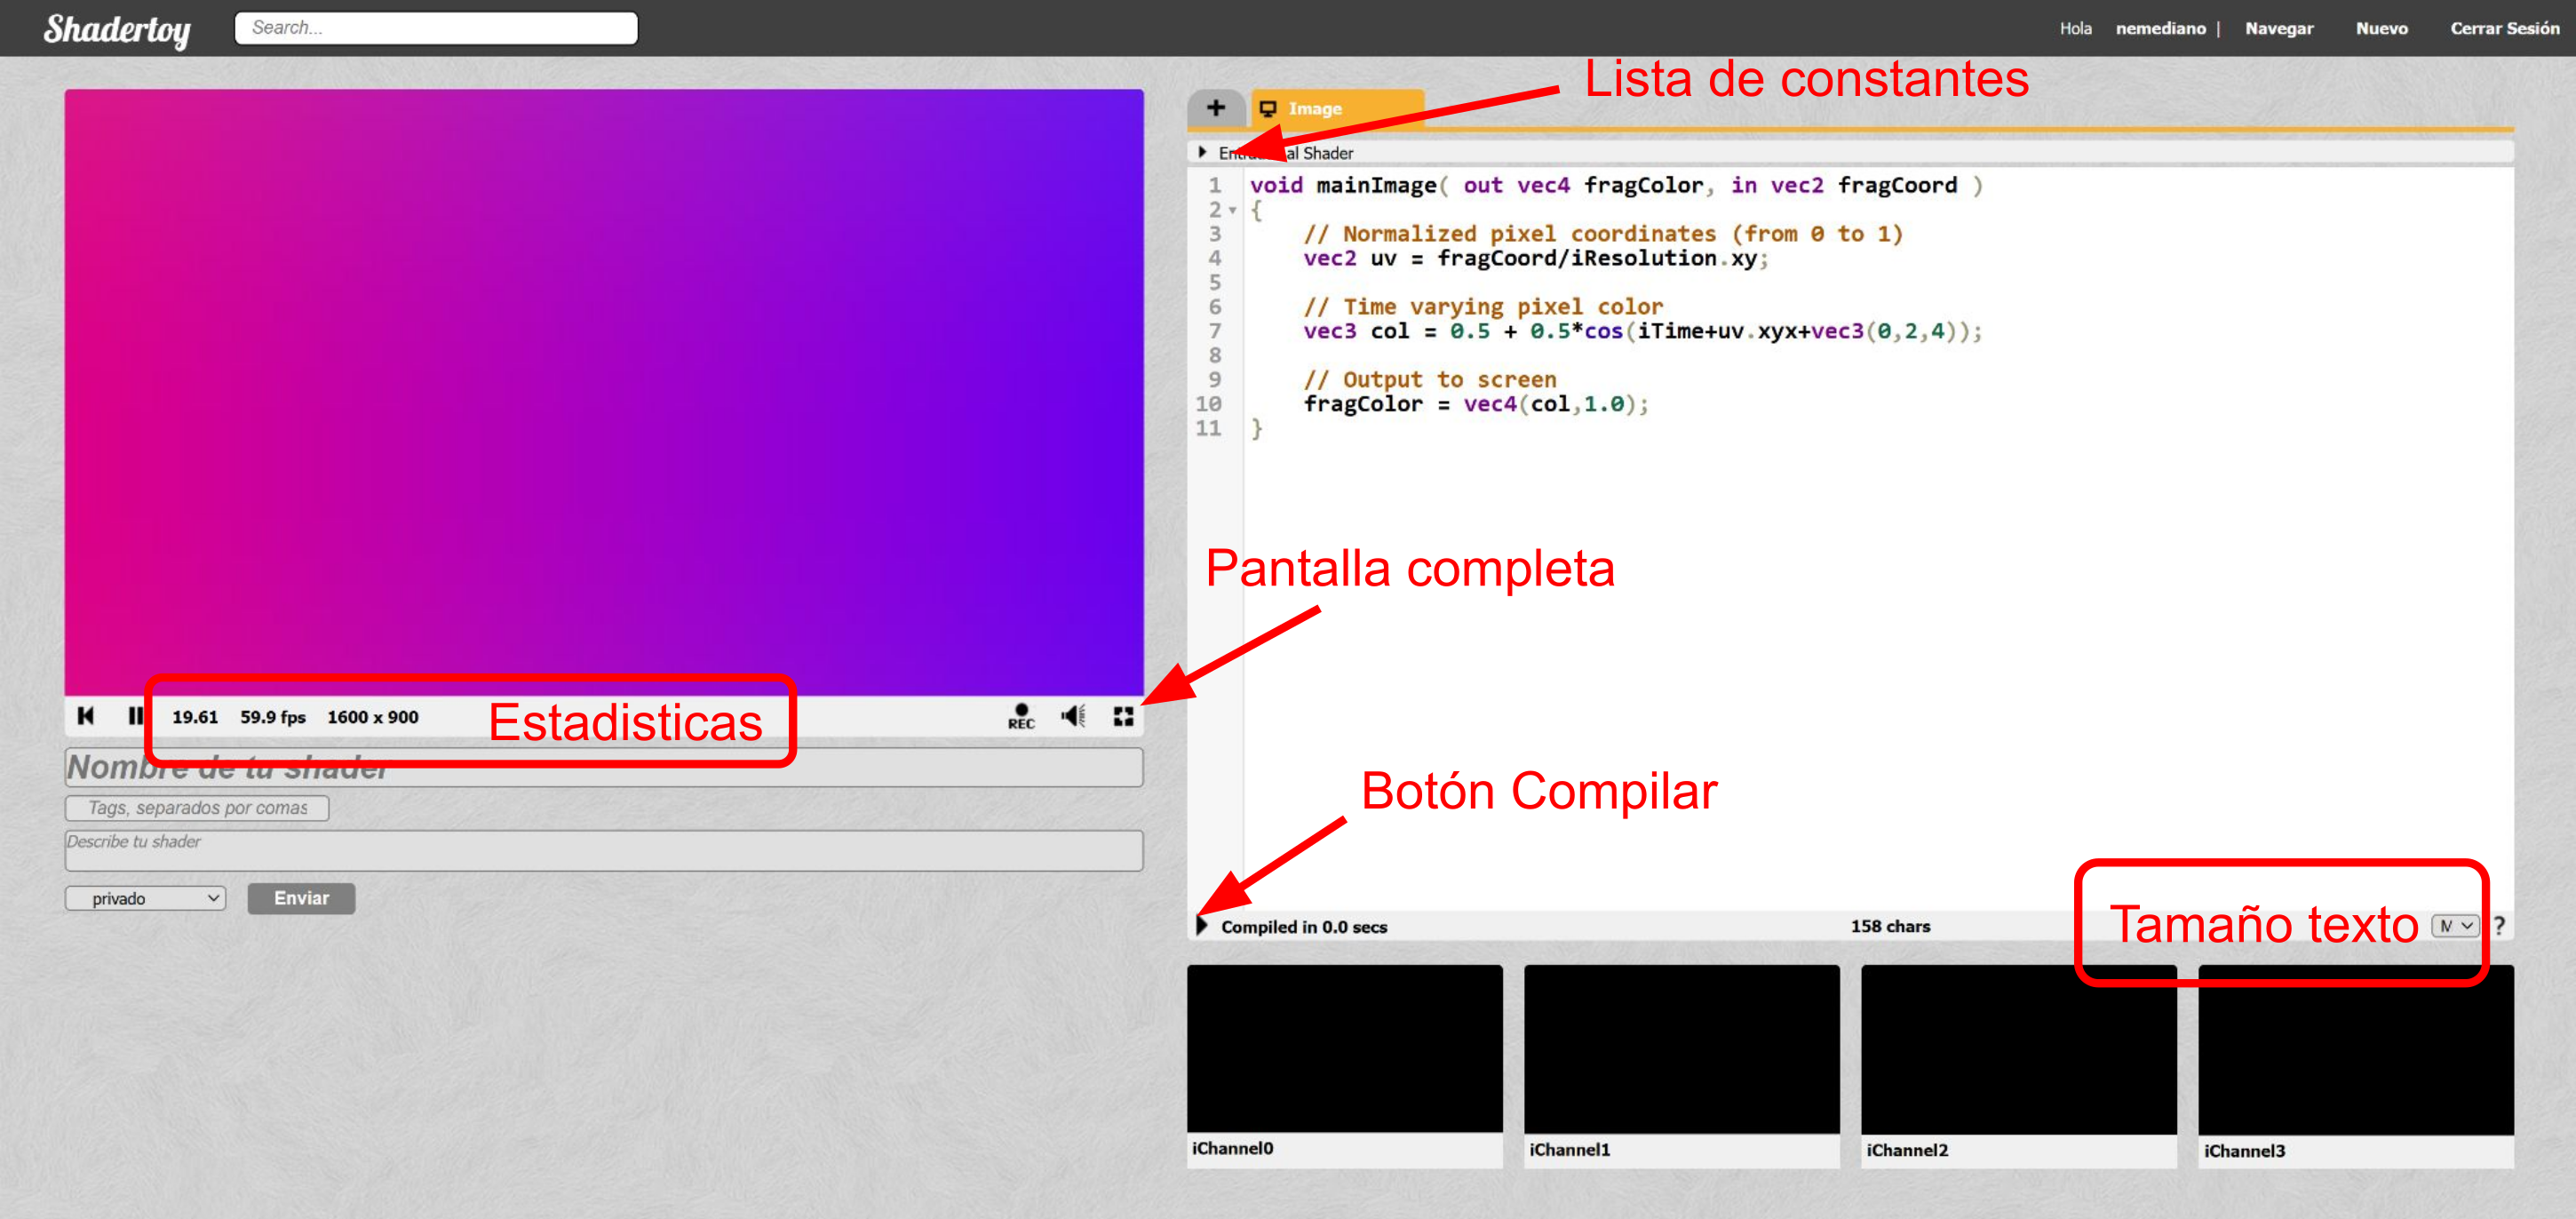
\includegraphics[width=0.8\textwidth]{img/ShaderToyUI}
\end{figure}
\end{frame}

\begin{frame}{Portabilidad}
Shadertoy:
\begin{itemize}
    \item Crea el pipeline por nosotros
    \item Inyecta código en el fragment shader
\end{itemize}
Pero ten por seguro que:
\begin{block}{}
    Cualquier shader que funciona en shadertoy, puede ser \alert{portado} y funcionar en cualquier otro entorno que pueda desplegar gráficos.
\end{block}
Adicionalmente:
\begin{itemize}{}
    \item Hay muchos entornos de programación, que emulan Shadertoy
    \item Siempre puedes escribir tu propio programa que ejecute shaders de shadertoy
\end{itemize}
\begin{block}{}
    No es tan difícil, cualquier alumno que haya tomado una clase de CG puede hacerlo fácilmente.
\end{block}
\end{frame}

\section{GLSL: Lenguaje para escribir shaders}

\begin{frame}[fragile]{Tipos primitivos}
Esta \alert{no es} una lista exhaustiva, ante la duda consulta la \href{https://www.khronos.org/opengl/wiki/Data_Type_(GLSL)}{referencia}.
\begin{itemize}
    \item Tipos de escalares: \mintinline{glsl}{float}, \mintinline{glsl}{int}, \mintinline{glsl}{bool}.
    \item Vectores de $n \in \{2, 3, 4\}$ dimensiones: \mintinline{glsl}{vec3}, \mintinline{glsl}{ivec2}, \mintinline{glsl}{bvec4}.
    \begin{itemize}
        \item Nótese que cuando el tipo subyacente es \mintinline{glsl}{float} no se requiere el prefijo.
    \end{itemize}
    \item Los operadores aritméticos entre vectores se aplican por componente.
    \begin{itemize}
        \item Requieren que los operandos sean del mismo tamaño
    \end{itemize}
    \item Matrices de $n\times m$ dimensiones donde $n, m \in \{2, 3, 4\}$ dimensiones: \mintinline{glsl}{mat2x3}, \mintinline{glsl}{mat3x4}.
    \begin{itemize}
        \item Todas las matrices son de tipo \mintinline{glsl}{float}
        \item Las matrices cuadradas se pueden abreviar: \mintinline{glsl}{mat2}
        \item Las operaciones entre matrices, son las esperadas del álgebra lineal
    \end{itemize}
    \item Las multiplicaciones: \say{matriz por matriz}, \say{matriz por vector}, \say{escalar por vector} y  \say{escalar por matriz} son las definida en álgebra lineal.
\end{itemize}

\end{frame}

\begin{frame}[fragile]{Swizzling}
\begin{itemize}
    \item Los tipos vectoriales tienen accesores y mutadores a sus componentes individuales.
    \item Los accesores tienen tres sintaxis equivalentes: $(x, y, z, w), (r, g, b, a), (s, t, p, q)$.
\end{itemize}
Esto define el llamado Swizzling:
\begin{listing}
\begin{minted}{glsl}
vec2 someVec;
vec4 otherVec = someVec.xyxx;
vec3 thirdVec = otherVec.zyy;
vec4 fourthVec;
// Tambien funciona en l-values:
fourthVec.wzyx = vec4(1.0, 2.0, 3.0, 4.0); // Reverses the order.
fourthVec.zx = vec2(3.0, 5.0); // Sets the 3rd component to 3 and the 1st component to 5
\end{minted}
\end{listing}
\end{frame}

\begin{frame}[fragile]{Constructores de vectores}
Se pueden construir a partir de:
\begin{itemize}
    \item Vectores de mayor dimensión (los componentes extra son ignorados).
    \item Una combinación de escalares y de vectores de menor dimensión.
    \item De manera abreviada, especificando un solo escalar que se repite.
\end{itemize}
\begin{listing}
\begin{minted}{glsl}
vec4(vec2(10.0, 11.0), 1.0, 3.5) == vec4(10.0, vec2(11.0, 1.0), 3.5);
vec3(vec4(1.0, 2.0, 3.0, 4.0)) == vec3(1.0, 2.0, 3.0);
vec4(vec3(1.0, 2.0, 3.0)); // error. Not enough components.
vec2(vec3(1.0, 2.0, 3.0)); // OK
vec3(1.0) // Abreviation to say: vec3(1.0, 1.0, 1.0);
\end{minted}
\end{listing}
\end{frame}


\begin{frame}[fragile]{Constructores de matrices}
\begin{itemize}
    \item Se construyen por columnas.
    \item Se pueden construir a partir de matrices de menor o igual dimensión.
    \item O de manera abreviada especificando un solo escalar que llena la diagonal.
\end{itemize}
\begin{listing}
\begin{minted}{glsl}
mat2(
  float, float,   // first column
  float, float);  // second column

mat4(
  vec4,           // first column
  vec4,           // second column
  vec4,           // third column
  vec4);          // fourth column

mat3 diagMatrix = mat3(5.0);  // Diagonal matrix with 5.0 on the diagonal.
mat4 otherMatrix = mat4(diagMatrix); // The last element on the diagonal is 1.0
\end{minted}
\end{listing}
\end{frame}

\begin{frame}{Built-in functions}
Además de las funciones habituales esperadas, algunas funciones interesantes:
\begin{table}[htb]
  \begin{center}
    \begin{tabular}{l | l }
      \mintinline{glsl}{vec3 mix(vec3 x, vec3 y, float a)} & Interpolación lineal \\
      \mintinline{glsl}{vec3 step(float edge, vec3 x)} & Función escalón \\
      \mintinline{glsl}{mat4 inverse(mat4 M)} & Matriz inversa \\
      \mintinline{glsl}{float dot(vec3 x, vec3 y)} & Producto punto \\
      \mintinline{glsl}{vec3 cross(vec3 x, vec3 y)} & Producto cruz \\
      \mintinline{glsl}{vec3 reflect(vec3 i, vec3 n)} & Reflejar $\mathbf{i}$ a partir de $\mathbf{n}$ \\
      \mintinline{glsl}{vec3 clamp(vec3 x, vec3 min, vec3 max)} & Limitar entre dos valores \\
      \mintinline{glsl}{float length(vec3 x)} & Norma de un vector \\
      \mintinline{glsl}{vec3 normalize(vec3 x)} & Vector normalizado \\
      \mintinline{glsl}{float distance(vec3 x, vec3 y)} & Distancia entre dos puntos \\
    \end{tabular}
  \end{center}
\end{table}
Todas las funciones tienen las sobrecargas vectoriales, cuando corresponde.
\end{frame}

\section{Mis primeros shader de juguete}
\begin{frame}{Repositorio}
Todo lo necesario para este taller esta en este repositorio: 
\begin{block}{}
\url{https://github.com/nemediano/tallerShadertoy}.
\end{block}
\begin{itemize}
    \item Ésta presentación, también esta en el mismo repositorio. Así puedes seguir los links.
    \item Para cada ejercicio, hay dos versiones de código fuente.
    \begin{enumerate}
        \item El código mínimo para empezar el ejercicio
        \item Una posible solución al ejercicio 
    \end{enumerate}
\end{itemize}

\end{frame}

\begin{frame}{Últimos detalles}
En shadertoy, la ejecución inicia y termina con la función:

\mintinline{glsl}{void mainImage(out vec4 fragColor, in vec2 fragCoord)}.

\begin{itemize}
    \item Por cada fragment recibes de parámetro: \mintinline{glsl}{fragCoord}, con la posición del fragment en el \emph{render target}.
    \item La salida: \mintinline{glsl}{fragColor}, es un output parameter. Un vector de dimensión 4 que debe contener el color final del fragment.
    \begin{itemize}
        \item La salida $\mathbf{x} \in \mathbb{R}^{4}$ debe tener $ x_i \in [0, 1]$.
        \item El último componente $x_4$ (ó bien $w$), representa el componente alpha, que en Shadertoy debe ser 1.
    \end{itemize}
\end{itemize}
\end{frame}

\begin{frame}{Ejercicio: Bandera a cuadros}
    \begin{columns}
\column[t]{0.5\textwidth}
     \begin{itemize}
         \item Tratar de escribir un shader que genere una bandera a cuadros (o tablero de ajedrez si lo prefieres)
         \item Puedes empezar con el código de default de shader toy.
         \item Recuerda las funciones trigonométricas
     \end{itemize}
\column[t]{0.5\textwidth}
        \begin{figure}[htb]
            \centering
            
\includegraphics[width=0.6\textwidth]{img/Ejer1}
            \caption{\url{https://github.com/nemediano}}
        \end{figure}
\end{columns}
\end{frame}


\subsection{Funciones de distancia}

\begin{frame}{Sistema de coordenadas}
\begin{columns}
\column[t]{0.5\textwidth}
    \begin{itemize}
         \item Al principio, las coordenadas del fragment están en el espacio del imagen del render target. Miden pixeles.
         \item Cuando dividimos entre la resolución del render target, están en coordenadas de textura ($uv$-mapping). $u,v \in [ 0,1 ]$
     \end{itemize}
\column[t]{0.5\textwidth}
\begin{figure}[htp]
 \centering
 \begin{subfigure}[b]{0.45\textwidth}
   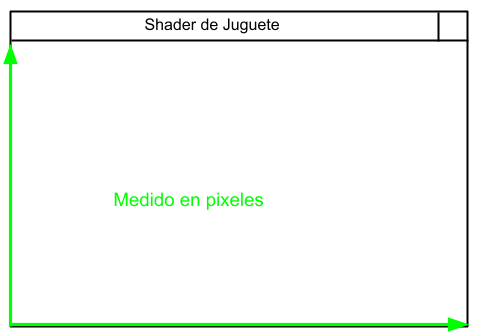
\includegraphics[width=\textwidth]{img/FrameOfreference}
   \caption{Espacio de imagen}
 \end{subfigure}
\\
 \begin{subfigure}[b]{0.45\textwidth}
   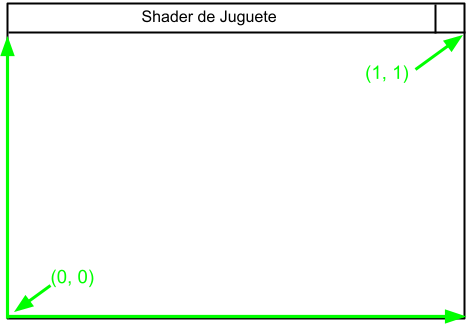
\includegraphics[width=\textwidth]{img/FoRUVSpace}
   \caption{$uv$ space}
 \end{subfigure}
\end{figure}
\end{columns}
\end{frame}

\begin{frame}{Sistema de coordenadas II}
\begin{columns}
\column[t]{0.5\textwidth}
    \begin{itemize}
        \item Cuando restamos 0.5 y multiplicamos por dos. Están en coordenadas normalizadas. $x,y \in [-1, 1]$.
        \item Cuando corregimos con el \emph{aspect ratio} de la pantalla, están en coordenadas de la escena. El origen esta en el centro, el eje mas restrictivo esta en $[-1, 1]$ y el otro es proporcional.
     \end{itemize}
\column[t]{0.5\textwidth}
\begin{figure}[htp]
 \centering
 \begin{subfigure}[b]{0.45\textwidth}
   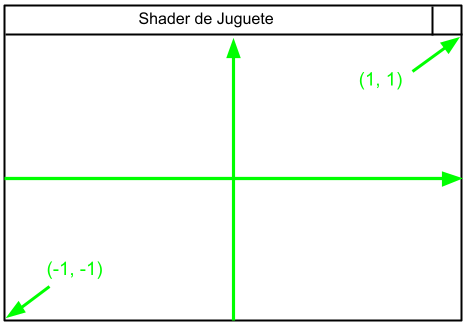
\includegraphics[width=\textwidth]{img/FoRNormalized}
   \caption{Normalize coordinates}
 \end{subfigure}
\\
 \begin{subfigure}[b]{0.45\textwidth}
   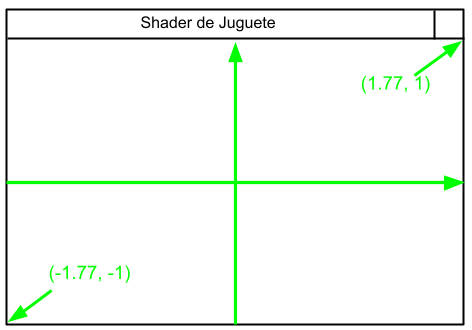
\includegraphics[width=\textwidth]{img/FoRCorrected}
   \caption{World Coordinates}
 \end{subfigure}
\end{figure}
\end{columns}
\end{frame}

\begin{frame}[fragile]{Función de transformación}
\begin{listing}
\begin{minted}{glsl}
vec3 getWorldCoordinates(vec2 fragCoord, vec3 iResolution) {

    float aspectRatio = iResolution.x / iResolution.y;

    vec2 scaleFactor =
        iResolution.x > iResolution.y ? vec2(aspectRatio, 1.0) : vec2(1.0, 1.0 / aspectRatio);

    vec2 world = scaleFactor * (2.0 * (fragCoord/iResolution.xy) - vec2(1.0));

    return vec3(world, 1.0);
}
\end{minted}
\end{listing}
Después veremos por que esta función, de hecho regresa un vector en $\mathbb{R}^3$, cuyo tercer componente es 1.
\end{frame}


\begin{frame}{Función de distancia con signo}

\begin{itemize}
    \item En Inglés mejor conocida como: \emph{signed distance field} (sdf).
    \item Hay una \href{https://en.wikipedia.org/wiki/Signed_distance_function}{definición formal}. Pero intuitivamente:
    \begin{itemize}
        \item Si tienes una curva cerrada $c$ en $\mathbb{R}^n$, cuya frontera es $\delta$.
        \item Entonces la $sdf(c)$ es una función continua $sdf: \mathbb{R}^n \rightarrow \mathbb{R}$, tal que es positiva en el exterior de $f$, negativa en el interior de $f$ y cero en $\delta$.
    \end{itemize}
\end{itemize}
\begin{columns}
\column[t]{0.4\textwidth}
     \begin{itemize}
         \item Para el circulo $x^2 + y^2 = 1$
         \item Una posible sdf es: $x^2 + y^2 - 1$
     \end{itemize}
\column[t]{0.6\textwidth}
        \begin{figure}[htb]
            \centering
            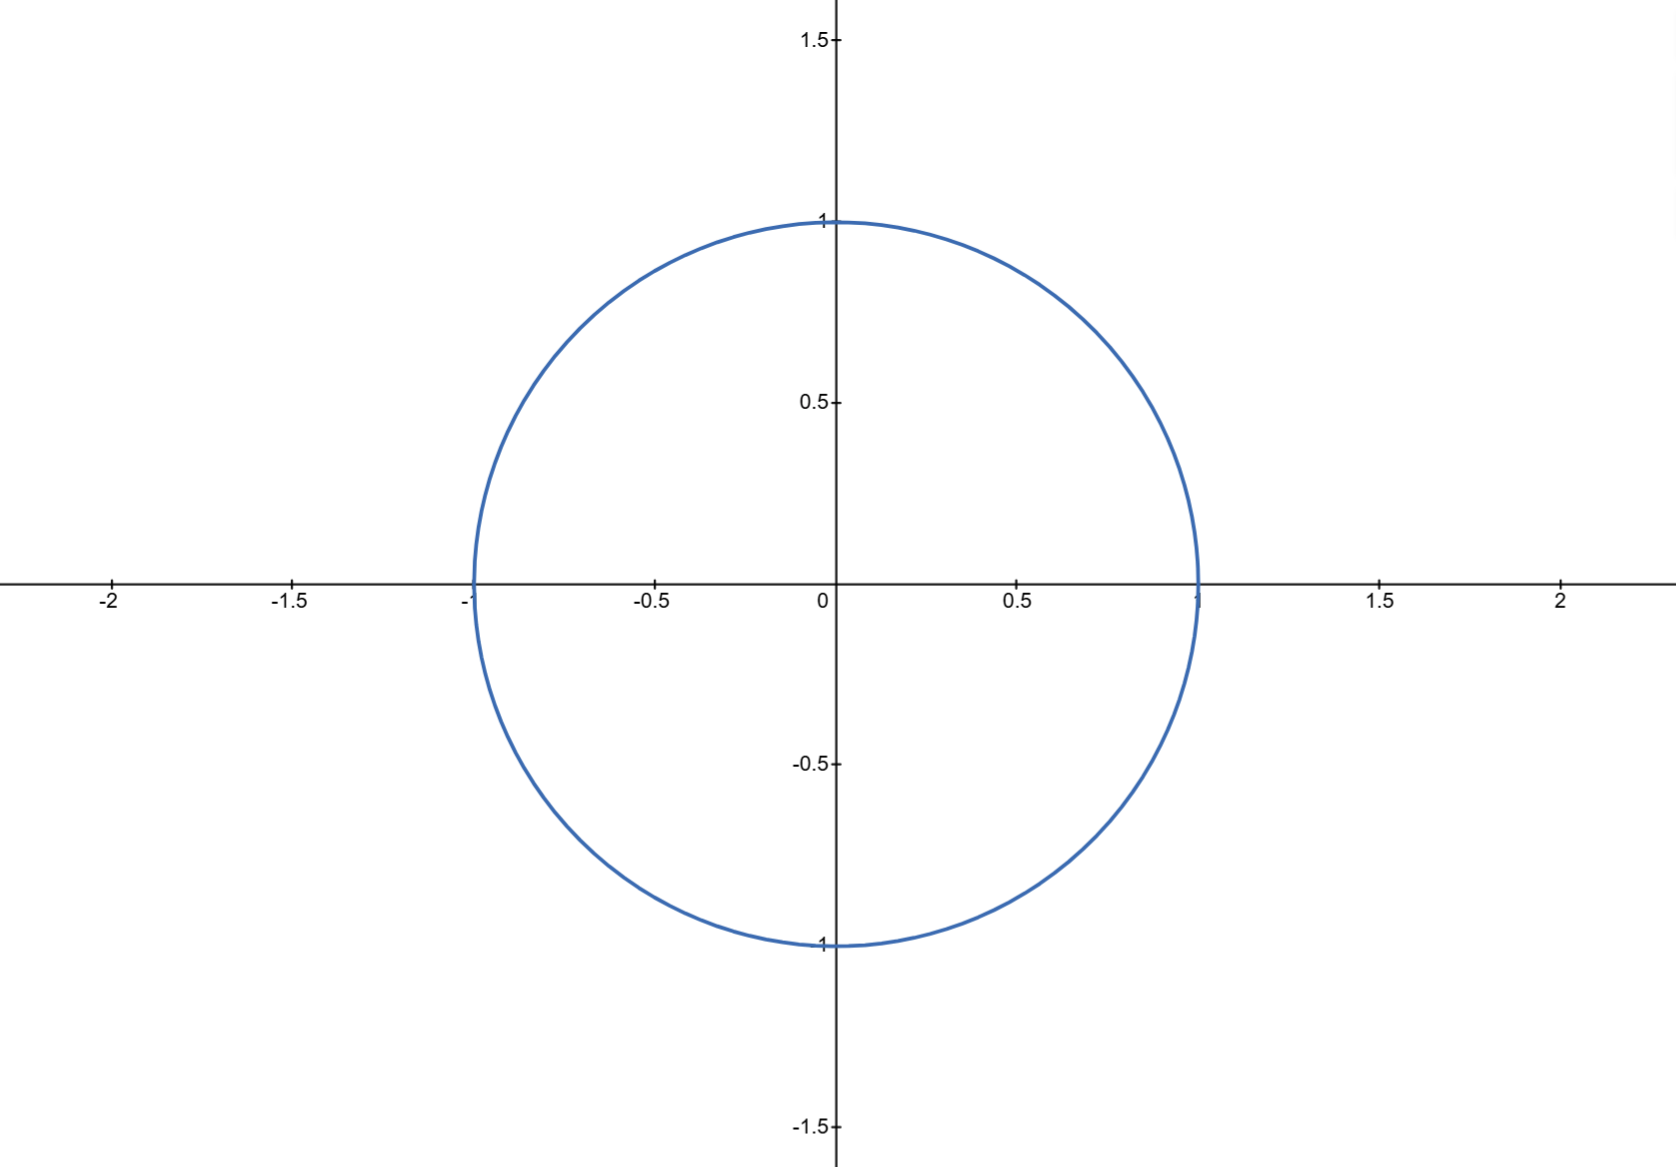
\includegraphics[width=0.6\textwidth]{img/unitCircle.png}
        \end{figure}
\end{columns}
\end{frame}

\begin{frame}{Ejercicio: Un cuadrado detrás de un circulo}
\begin{columns}
\column[t]{0.5\textwidth}
     \begin{itemize}
         \item Abstraer el código en funciones
         \item Tener una función que cambia las coordenadas
         \item Tener una función para el fondo
         \item Puedes utilizar la guía de colores
     \end{itemize}
\column[t]{0.5\textwidth}
        \begin{figure}[htb]
            \centering
            
\includegraphics[width=0.6\textwidth]{img/Ejer2}
            \caption{\url{https://github.com/nemediano}}
        \end{figure}
\end{columns}
\end{frame}

\begin{frame}{Transformaciones Afines}
Hay una definición formal de \href{https://en.wikipedia.org/wiki/Affine_transformation}{transformación afín}. Pero para nuestros propósitos, podremos decir que: una transformación afín $A: \mathbb{R}^n \rightarrow \mathbb{R}^n$ es una transformación lineal seguida de una traslación.

\begin{block}{}
    Si $\mathbf{x} \in \mathbb{R}^n$, $M$ es una matriz de $n \times n$ y $\mathbf{d} \in \mathbb{R}^n$ un vector.
    Entonces $A(\mathbf{x}) = M \mathbf{x} + \mathbf{d}$ es una transformación afín.
\end{block}
\begin{itemize}
    \item Todas las transformaciones lineales son transformaciones afines (con $\mathbf{d} = \mathbf{0}$)
    \item Todas las traslaciones son transformaciones afines (con $M = I$).
\end{itemize}
\end{frame}


\begin{frame}{Coordenadas homogéneas}

\begin{itemize}
    \item Todas las transformaciones lineales pueden llevarse a cabo multiplicando matrices.
    \item Pero las traslaciones no se pueden llevar a cabo multiplicando matrices
    \item Para solucionar ese problemas usamos las \href{https://en.wikipedia.org/wiki/Homogeneous_coordinates}{coordenadas homogéneas}
\end{itemize}
Vamos a adoptar la convención de que tanto puntos, como vectores son representados en columna.
\begin{block}{}
    Las coordenadas homogéneas de un punto $\mathbf{x} \in \mathbb{R}^n$, son una tupla de $n+1$ componentes, formada por los $n$ componentes de $\mathbf{x}$, seguidos por el escalar 1.
\end{block}
Ésta \emph{no es} la definición general, pero hará las explicaciones mas sencillas.
\begin{itemize}
    \item Las coordenadas homogéneas representan al punto $\mathbf{x} \in \mathbb{R}^n$ con un punto $\mathbf{x}_{h} \in \mathbb{R}^{n+1}$.
    \item Pero permiten \emph{expresar las transformaciones afines como una multiplicación de matrices}.
\end{itemize}

\end{frame}

\begin{frame}{Traslación}
\begin{columns}
\column[t]{0.5\textwidth}
\begin{itemize}
    \item Traslada una curva en el espacio
    \item Tiene parámetro el vector de traslación $\mathbf{t}$
    \item Se puede expresar con la siguiente matriz:
\end{itemize}
$$
\begin{pmatrix}
1 & 0 & t_x\\
0 & 1 & t_y\\
0 & 0 & 1
\end{pmatrix}
\begin{bmatrix}
x \\
y \\
1 \\
\end{bmatrix}
=
\begin{bmatrix}
x + t_x \\
y + t_y \\
1 \\
\end{bmatrix}
$$
\begin{itemize}
    \item Si $\mathbf{t} = \mathbf{0}$, hay una operación nula
    \item La operación inversa es trasladar por $-\mathbf{t}$
    \item La figura muestra una traslación por $\mathbf{t} = (2, 1)^t$
\end{itemize}
\column[t]{0.5\textwidth}
\begin{figure}[htp]
 \centering
 \begin{subfigure}[b]{0.4\textwidth}
   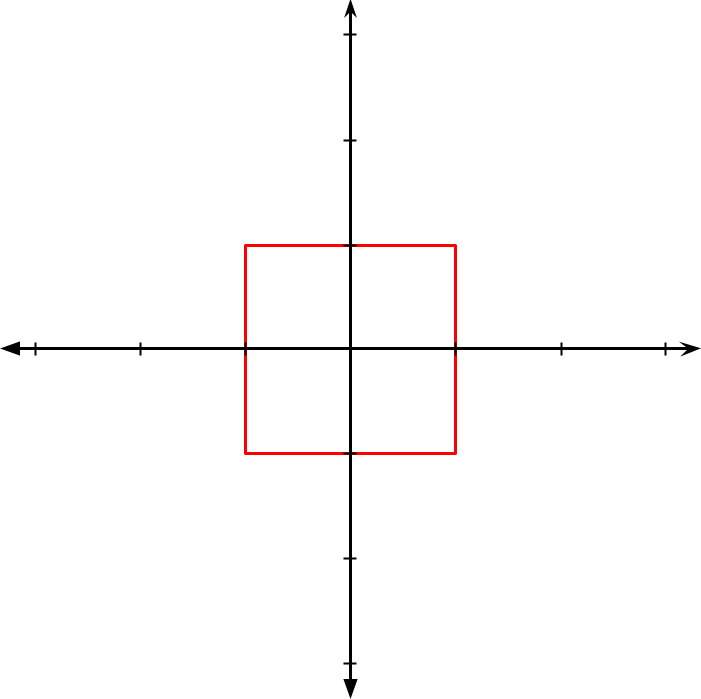
\includegraphics[width=\textwidth]{img/Square}
 \end{subfigure}
\\
\vspace{0.15cm}
 \begin{subfigure}[b]{0.4\textwidth}
   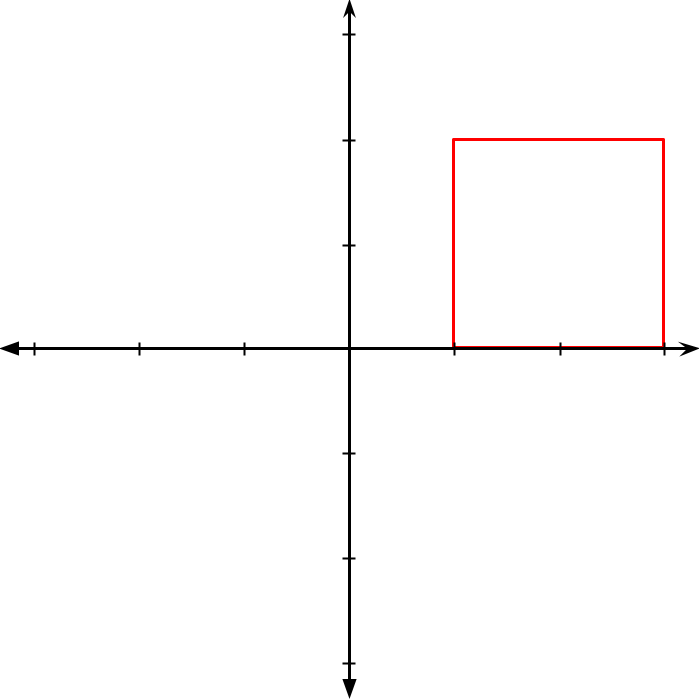
\includegraphics[width=\textwidth]{img/Translated}
 \end{subfigure}
\end{figure}
\end{columns}
\end{frame}

\begin{frame}{Rotación}
\begin{columns}
\column[t]{0.5\textwidth}
\begin{itemize}
    \item Rota una curva \emph{alrededor del origen}
    \item Tiene parámetro el angulo de rotación $\theta$
    \item Se puede expresar con la siguiente matriz:
\end{itemize}
$$
\begin{pmatrix}
\cos \theta & -\sin \theta & 0 \\
\sin \theta & \cos \theta & 0 \\
0 & 0 & 1
\end{pmatrix}
\begin{bmatrix}
x \\
y \\
1 \\
\end{bmatrix}
=
\begin{bmatrix}
x \cos \theta - y \sin \theta \\
x \sin \theta + y \cos \theta  \\
1 \\
\end{bmatrix}
$$
\begin{itemize}
    \item Si $\theta = 0$, hay una operación nula
    \item La operación inversa es rotar por $-\theta$
    \item La figura muestra una rotación de $\theta = \frac{\pi}{4}$
\end{itemize}
\column[t]{0.5\textwidth}
\begin{figure}[htp]
 \centering
 \begin{subfigure}[b]{0.4\textwidth}
   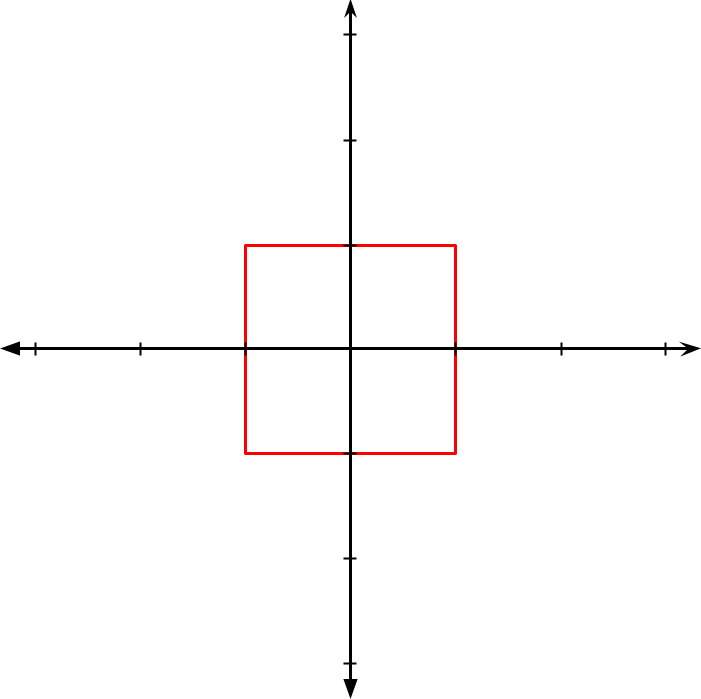
\includegraphics[width=\textwidth]{img/Square}
 \end{subfigure}
\\
\vspace{0.15cm}
 \begin{subfigure}[b]{0.4\textwidth}
   
\includegraphics[width=\textwidth]{img/Rotated}
 \end{subfigure}
\end{figure}
\end{columns}
\end{frame}

\begin{frame}{Escalamiento}
\begin{columns}
\column[t]{0.5\textwidth}
\begin{itemize}
    \item Escala una curva \emph{con respecto al origen}
    \item Tiene parámetro el factor de escala $\mathbf{s}$
    \item Se puede expresar con la siguiente matriz:
\end{itemize}
$$
\begin{pmatrix}
s_x & 0 & 0 \\
0 & s_y & 0 \\
0 & 0 & 1
\end{pmatrix}
\begin{bmatrix}
x \\
y \\
1 \\
\end{bmatrix}
=
\begin{bmatrix}
s_x \cdot x  \\
s_y \cdot y  \\
1 \\
\end{bmatrix}
$$
\begin{itemize}
    \item Si $\mathbf{s} = ( 1 , 1 )^t$, hay una operación nula
    \item La operación inversa es escalar por $\mathbf{s} = (\frac{1}{s_x} , \frac{1}{s_y} )^t$
    \item La figura muestra un escalamiento por $\mathbf{s} = ( \frac{1}{2} , 2 )^t$
\end{itemize}
\column[t]{0.5\textwidth}
\begin{figure}[htp]
 \centering
 \begin{subfigure}[b]{0.4\textwidth}
   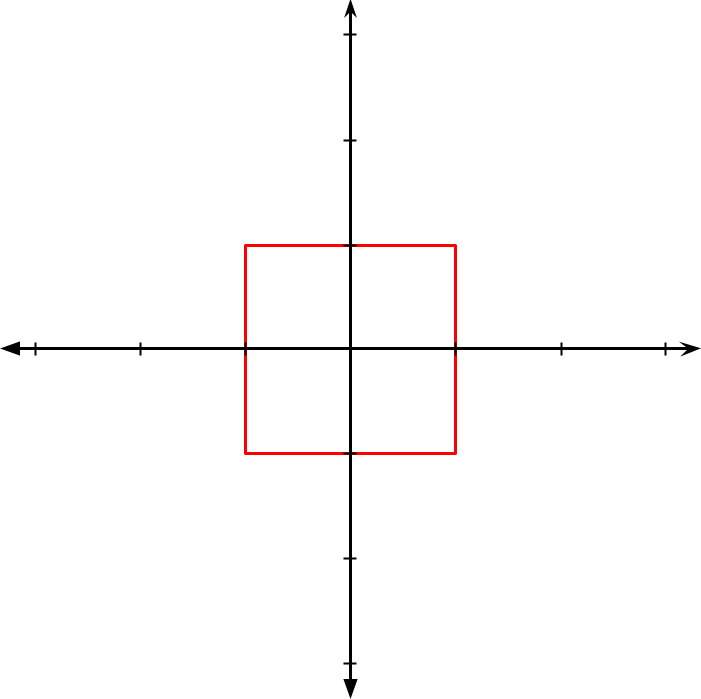
\includegraphics[width=\textwidth]{img/Square}
 \end{subfigure}
\\
\vspace{0.15cm}
 \begin{subfigure}[b]{0.4\textwidth}
   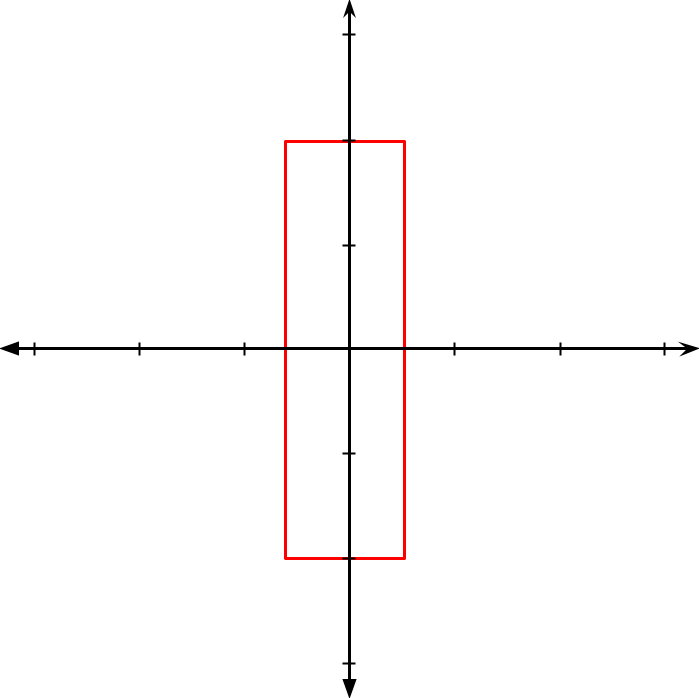
\includegraphics[width=\textwidth]{img/Scalated}
 \end{subfigure}
\end{figure}
\end{columns}
\end{frame}

\begin{frame}{Composición de transformaciones afines}
Las transformaciones afines, se pueden aplicar una después de otra. 
\begin{itemize}
    \item Esto se llama \alert{composición de transformaciones}
    \item Y es particularmente útil que se haga con matrices
    \item La multiplicación de matrices es asociativa 
    $$T_1 T_2 T_3 \mathbf{x} = T_1 (T_2 (T_3 \mathbf{x})) = (T_1 T_2 T_3) \mathbf{x}$$
    \item La multiplicación de matrices no es conmutativa: 
    $$T_1 T_2 \mathbf{x} \neq T_2 T_1 \mathbf{x}$$
\end{itemize}
\end{frame}

\begin{frame}{Ejemplo}
Si $R$ fuera una rotación de $\frac{5\pi}{4}$ y $S$ escalameinto por $(\frac{1}{2}, 2)^t$
\begin{figure}[htp]
 \centering
 \begin{subfigure}[b]{0.25\textwidth}
   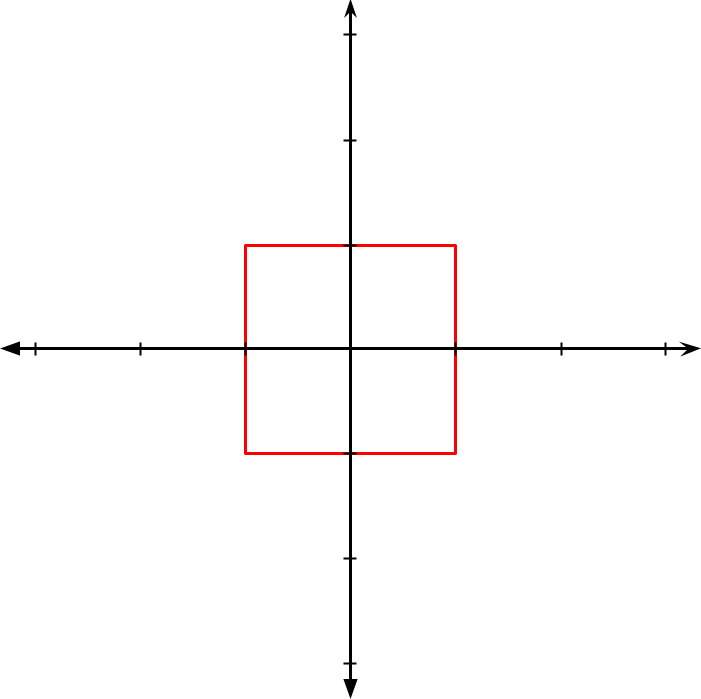
\includegraphics[width=\textwidth]{img/Square}
   \caption{Figura original}
 \end{subfigure}
 ~
 \begin{subfigure}[b]{0.25\textwidth}
   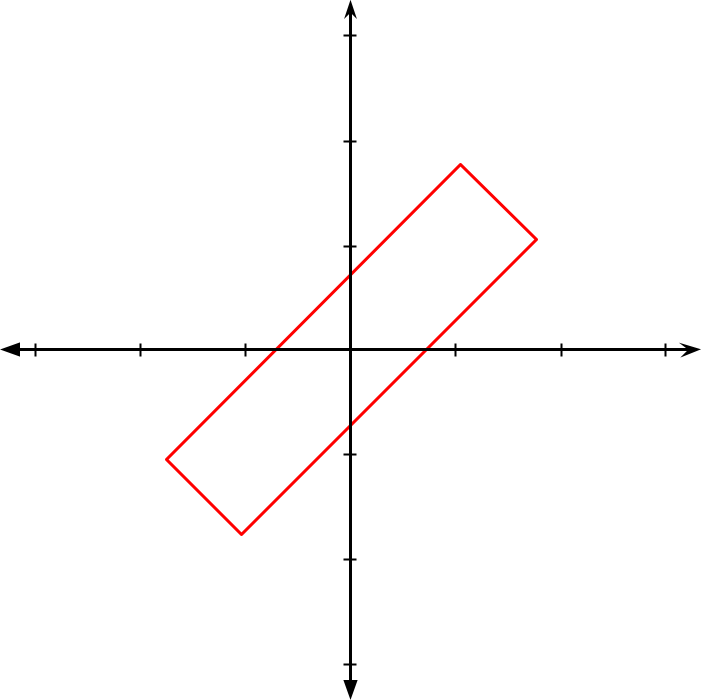
\includegraphics[width=\textwidth]{img/ScaleRoate}
   \caption{$R S \mathbf{x} = ( R ( S \mathbf{x}))$}
 \end{subfigure}
 ~
 \begin{subfigure}[b]{0.25\textwidth}
   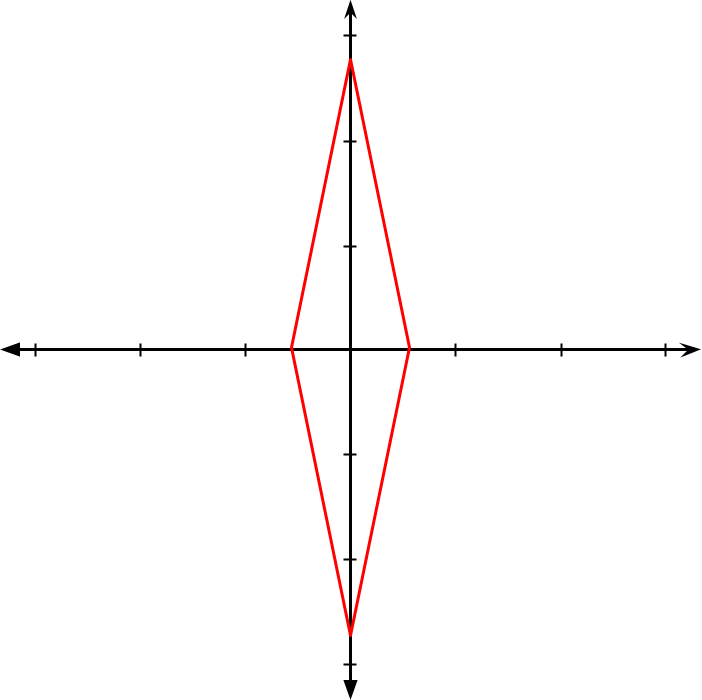
\includegraphics[width=\textwidth]{img/RoateScale}
   \caption{$S R \mathbf{x} = (S (R \mathbf{x}))$}
 \end{subfigure}
\end{figure}
\end{frame}

\begin{frame}{Transformaciones afines en Shadertoy}
\begin{itemize}
    \item La explicación anterior es como se hacen las gráficas tradicionalmente.
    \item Es decir, transformamos la geométrica para acomodarla en el espacio.
\end{itemize}
\begin{alertblock}{En Shadertoy en 2D hacemos lo contrario}
    \begin{itemize}
        \item En shadertoy en 2D, trasformamos las coordenadas del fragment hacia la figura.
        \item Esto es equivalente a decir que transformamos el espacio hacia la figura.
        \item Por lo tanto, para situar figuras en 2D usamos la matriz inversa de la matriz de trasformación.
    \end{itemize}
\end{alertblock}
\end{frame}

\begin{frame}[fragile]{Ejemplo en Shadertoy 2D}
\begin{listing}
\begin{minted}{glsl}
mat3 M = translate(vec2(0.75, 0.0)) * scale(vec2(0.25));

float disCircle = sdfCircle(inverse(M) * coord);

color = mix(Red, color, step(0.0, disCircle));
\end{minted}
\end{listing}
\begin{itemize}
    \item En este ejemplo se escala y luego se traslada una figura (circulo)
    \item Nótese la inversión de la matriz, antes de evaluar las sdf.
    \item Y el uso de la función \mintinline{glsl}{step} dentro de la función \mintinline{glsl}{mix}, para cambiar el color del fragment si estaba dentro de la figura.
\end{itemize}
\end{frame}

\begin{frame}{Ejercicio: Figuras animadas}
\begin{columns}
\column[t]{0.5\textwidth}
     \begin{itemize}
         \item Usar transformaciones compuestas para crear una escena
         \item Puedes utilizar la \href{https://iquilezles.org/articles/distfunctions2d/}{esta lista} para ver mas figuras
         \item Puedes comenzar con el código del ejercicio anterior 
     \end{itemize}
\column[t]{0.5\textwidth}
        \begin{figure}[htb]
            \centering
            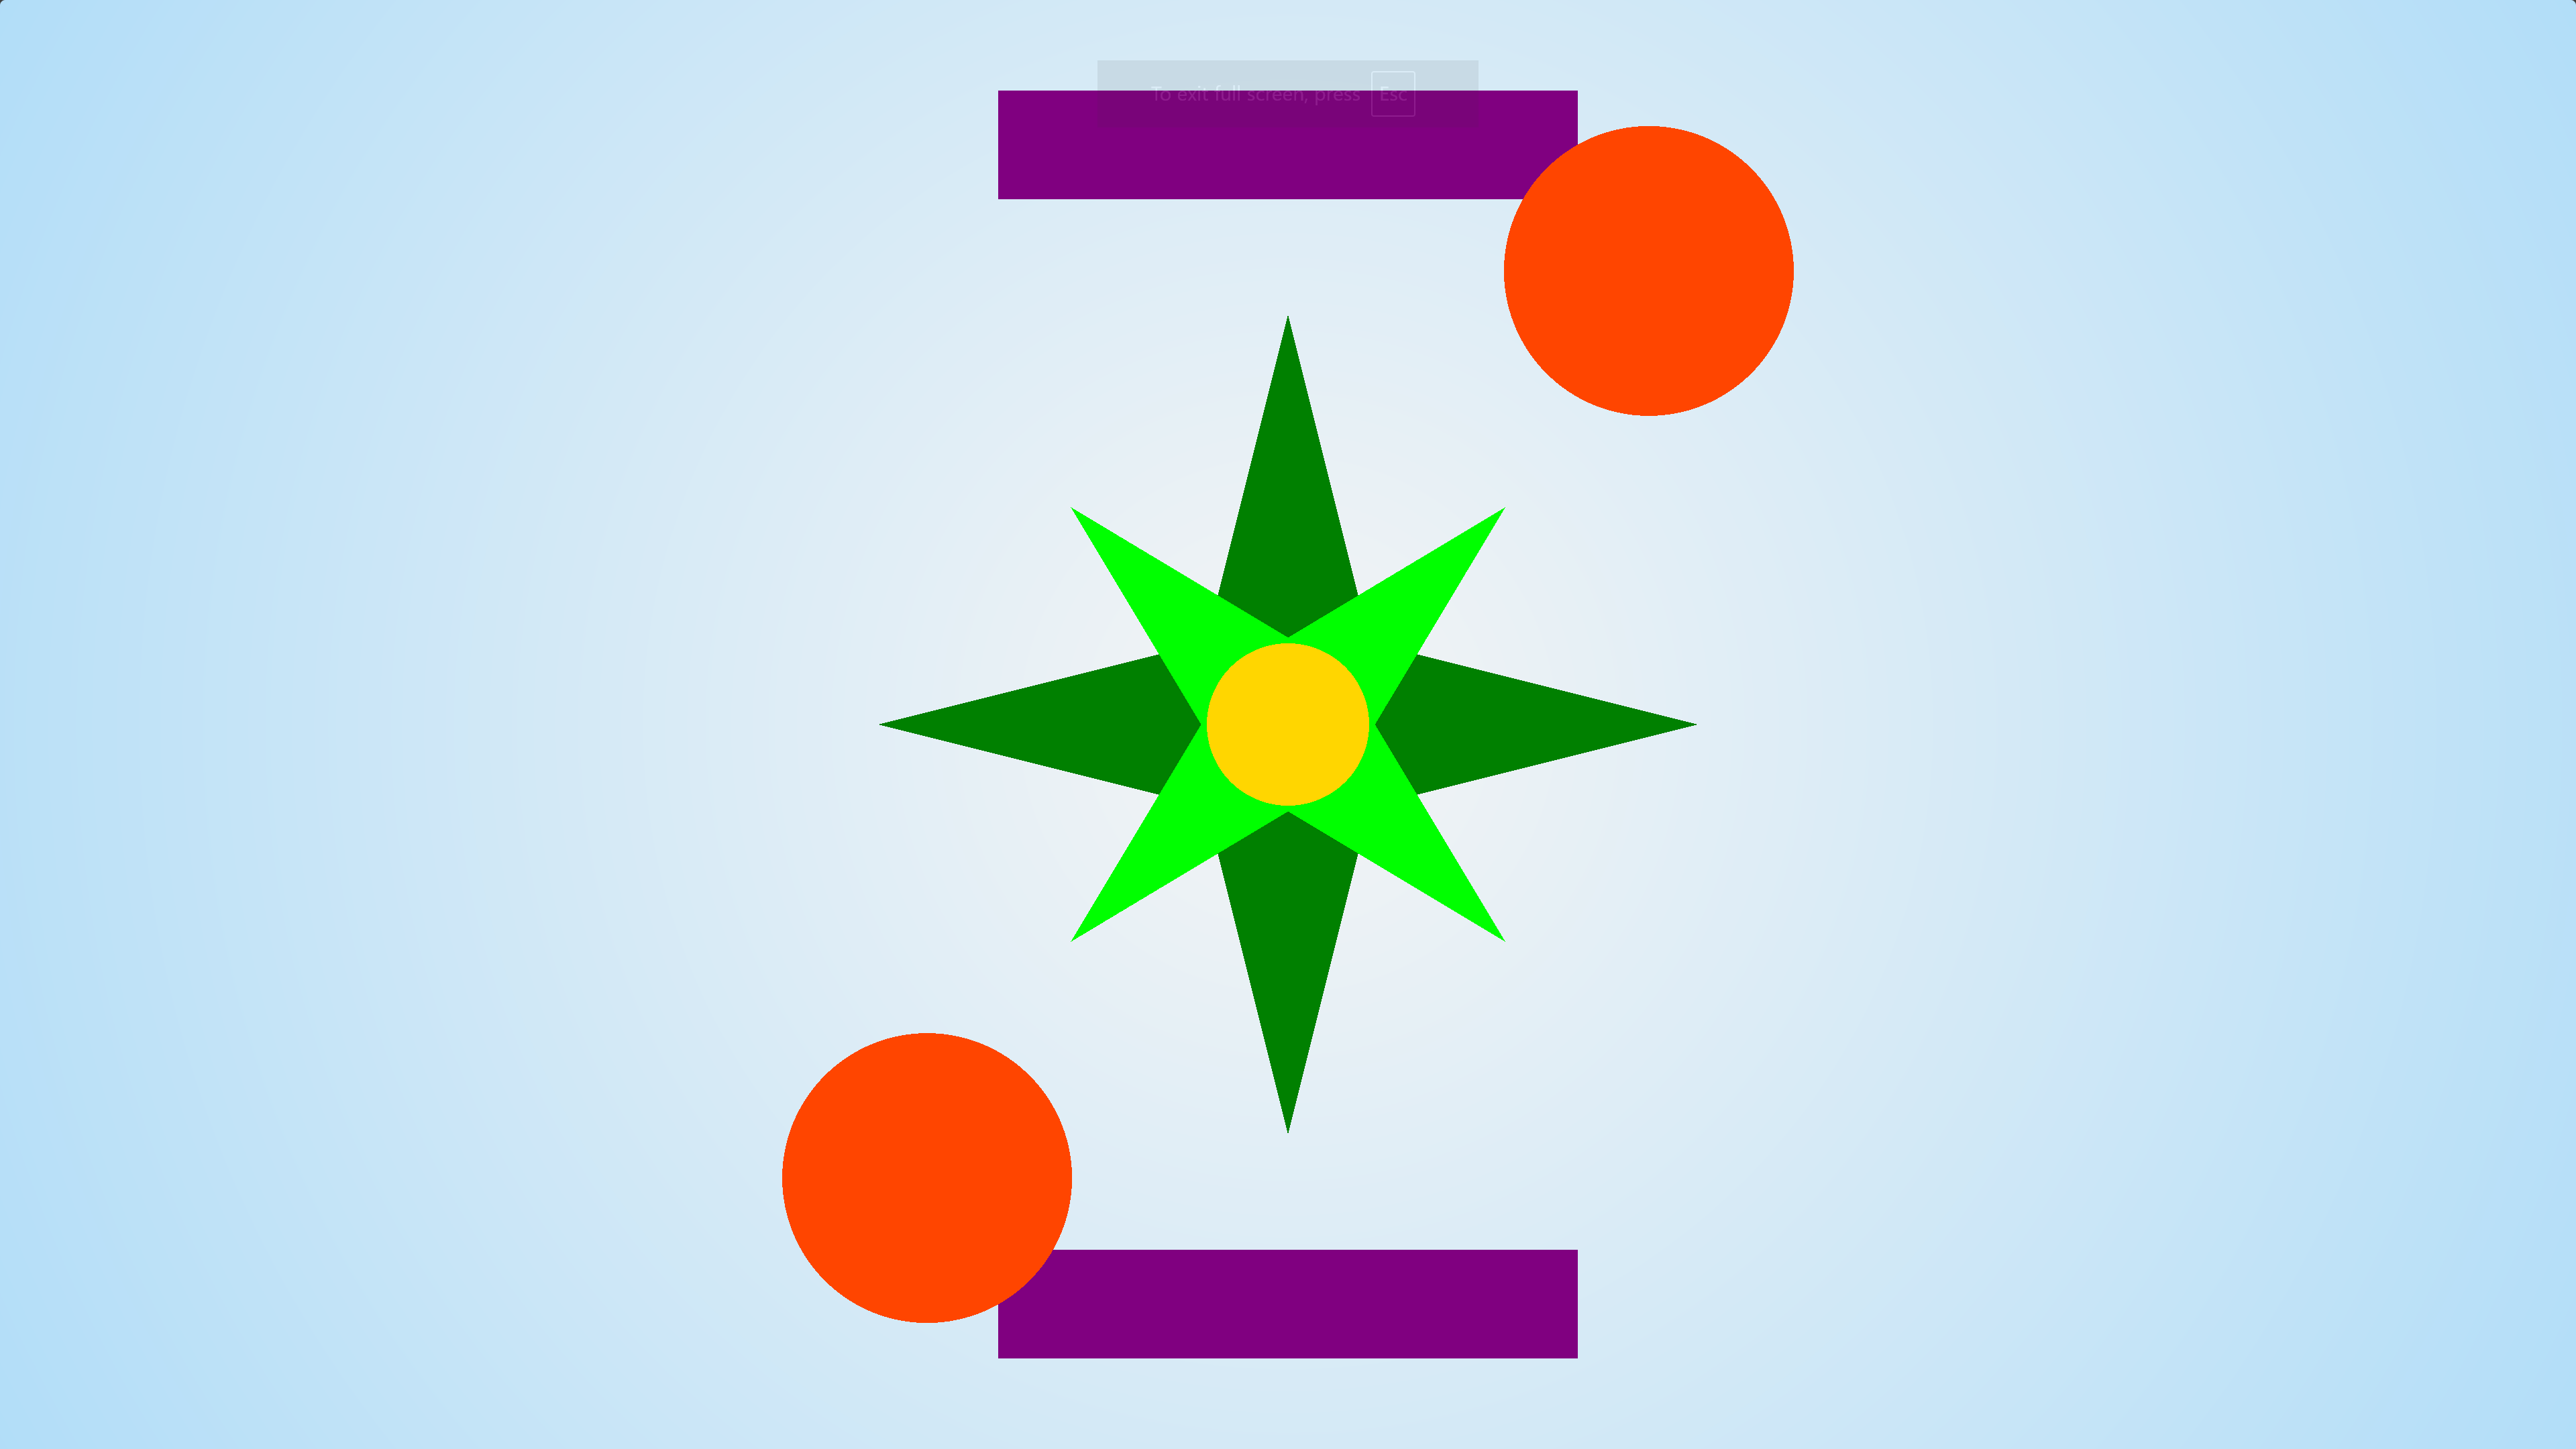
\includegraphics[width=0.6\textwidth]{img/Ejer3}
            \caption{\url{https://github.com/nemediano}}
        \end{figure}
\end{columns}
\end{frame}


\end{document}
